\chapter{Language strategies for humanoid robots}

This chapter discusses additional language game experiments directly inspired by the Talking Heads experiment, 
set up after 2005. Major breakthroughs along several dimensions have been achieved. Robots became hugely 
more complex, with humanoid shapes, and going from a few degrees of sensing and actuation to close to a hundred. The grammar 
formalisms developed for language game experiments matured, specifically the Fluid Construction Grammar formalism, developed 
as a successor of the \textsc{cogar} formalism reported in the previous chapter.\footnote{
A full introduction into Fluid Construction Grammar \is{Fluid Construction Grammar} 
is beyond the scope of this book. The interested reader is 
referred to the following two paper collections: \cite{Steels:2011} and \cite{Steels:2012}.}
Semantics was scaled up from propositional and predicate logic to fully open-ended procedural semantics.
And last but not least the theory of semiotic dynamics received a major impetus when statistical physicists became seriously 
involved, applying techniques and methods from complex systems science to study language game
dynamics, \cite{Loreto:2007}. \is{semiotic dynamics}
A large number of contributions were made by Loreto's Statistical Physics group at the University of Rome (La Sapienza), 
see in particular: \cite{DallaAsta:2006} and \cite{Baronchelli:2012}.
A full overview of all these developments is beyond the 
scope of this book. Instead we only look here at developments that directly pertain to language game experiments with robots. 

While introducing these experiments I will highlight two conceptual breakthroughs: semiotic networks and language strategies. 
\begin{itemize}
\item A {\scshape semiotic network} consists of a weighted network that links words to concepts, concepts to prototypes, and prototypes to 
sensory experiences. Each agent constructs his own semiotic network but through consecutive 
interactions these networks become progressively similar. From this perspective, setting up a language game requires a definition and 
operationalisation how new nodes are created in this network, how new links are made between 
the nodes, and how the weights between nodes are adjusted. 
\item A {\scshape language strategy} is helpful to think about how we can go beyond individual words and towards 
more complex grammatical expressions. It was already introduced in the previous chapter. 
A language strategy is a particular way to deal syntactically and semantically 
with one domain of meaning. It includes ways for conceptualising, expressing, acquiring and expanding a specific domain. 
For example, the colour domain requires not only strategies for basic colour terms (like \smplenquote{blue}), but also for 
graded membership expressions (\smplenquote{very blue}), composite colours, (\smplenquote{greenish blue}), analogical colours (\smplenquote{sky blue}), a.o. 
The Talking Heads experiments used a single strategy that was entirely hard-coded: discrimination trees for categorisation 
and words without syntax to express distinctive categories. Research efforts moved towards the study of other strategies, and 
to the question how such strategies may arise (discussed in the next chapter). 
\end{itemize}
The remainder of the present chapter illustrates these two notions through different language game experiments: The Proper 
Naming Game and the Action Naming Game illustrate the use of semiotic networks. The Colour Description Game and the 
Spatial Language Game illustrate the use of language strategies. These experiments also show how the focus of research 
progressively moved towards the emergence of grammar in co-evolution with more complex compositional, but still 
grounded, semantics. 

\section{The Proper Naming Game}

Around 2005, the same team that had built the \textsc{aibo} robot at the Sony Corporation central laboratories, managed to 
make another enormous leap forward by building \is{Proper Naming Game}
the \textsc{qrio} humanoid robot. This robot is about 60 cm tall and weighs 7.3 kg. Its sensors
include two cameras in the head, a microphone, and sensors in each motor joint to monitor posture and movement. The robot has enough
computing power and battery to autonomously walk around on its two legs and perform various actions in the world.
The \textsc{qrio} never made it to a commercial product for economical reasons. However, we were able to use \textsc{qrio} robots to 
carry out a series of ground-breaking experiments that without doubt pushed the state of the art in language games
forward considerably. 
The teleportation infrastructure developed for the original Talking Heads experiment was used again 
to allow experiments with populations of agents, despite having only a few robotic bodies available. 
For every game, two agents were downloaded into the on-board memory and processors 
of the \textsc{qrio} robot and after a game, the state of the agent was uploaded back to a central server. Agents never
interacted without being physically instantiated in the world. 

Initially the experiments were very close to the Talking Heads experiments but progressively 
they tackled more and more challenging semantic domains
including action description, spatial expressions, and quantifiers, and consequently
the complexity of the grammar increased. This section discusses one of the first experiments, namely 
for the emergence of a vocabulary of proper names, i.e. names for individuals.

In January 2007, Luc Steels, Martin Loetzsch, and Michael Spranger travelled to the Sony Computer Science Laboratory 
in Tokyo to do the first experiments with the \textsc{qrio} robots.  
We decided to redo the Talking Heads experiment, but focusing on proper names for individual objects, rather than the emergence 
of generic terms such as colours, shapes or positions.\enlargethispage{1\baselineskip}\footnote{The first paper on the Proper Naming Game is: \cite{Steels:2007}
It also discusses the concept of a semiotic network. 
A more recent paper is: \cite{Steels:2012b}. A more 
in-depth discussion of the experiment is included 
in the Ph.D thesis of Martin Loetzsch, defended in 2014 at Humboldt University.}

We also introduced games with multiple turns: While the agents were looking, we 
changed the environment for them, for example putting down a standing block so that 
agents could learn the appearance of object from different perspectives and in different positions. 
Not many changes were made to the Naming Strategy itself. The 
lateral inhibition strategy of the Talking Heads experiment was entirely adequate. The big issue was how to 
identify and consistently recognise objects as individuals and to figure out how language could help agents to do so. 

The general set-up for the Proper Naming Game experiment
is shown in \figref{fig:grounded}. We see two \textsc{qrio} robots and an environment consisting of objects of various 
sizes and shapes. At any time a new object can be added or the position of an object can be changed. So the world is 
entirely open and robots do not know how many individuals there are. 
Importantly, the robots had to recognise an object as an individual, independently of its position. If 
a specific object disappeared from the world and was put back later, the same name would still have to be used.

\begin{figure}[htbp]
  \centerline{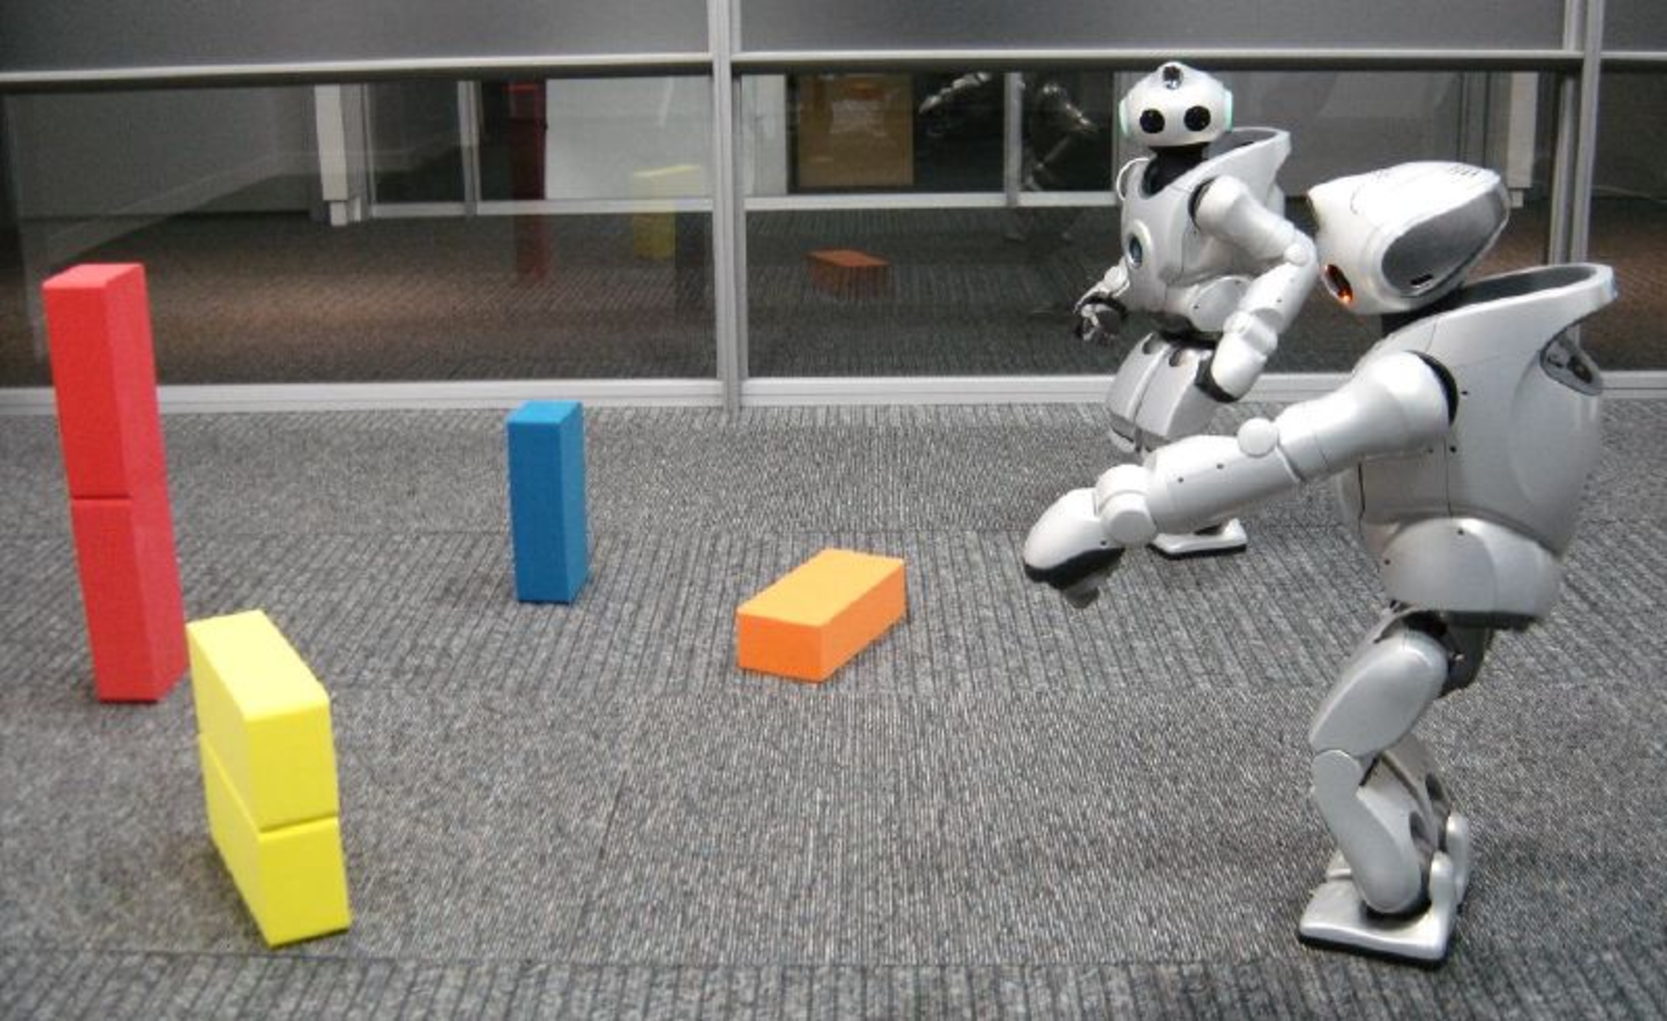
\includegraphics[width=.80\textwidth]{chap11/figs/grounded-naming-game.pdf}}
\caption{\label{fig:grounded}Set-up for the Grounded Proper Naming Game. Two Qrio robots are playing a game of reference about individual objects 
in their environment. They are using proper names and hence have to recognise objects as individuals.}
\end{figure}

\subsection{Challenges}
% {\bfshape Challenges} \\

It is useful to emphasise how extraordinary difficult this task is, even though the Talking Heads experiment and 
earlier experiments with the \textsc{aibo} already 
provided a good foundation. These difficulties are encountered for communication within any group of
autonomous physically embodied agents and hence also humans. 
First of all it is extremely challenging to set up joint-attention frames with free roaming
robots, which may explain why no other animals except humans can self-organise
shared symbolic systems. For the Proper Naming Game experiment, a robot moves around until another robot comes into 
view and remains sufficiently 
stationary. Both robots follow this strategy and so sooner or later a pair of robots find each other
and a game becomes possible. Next the robots both scan their immediate environment and build up an initial world model. 
They keep tracking the environment because it may change as games are being played. 
Because the robots can detect each other, they can reconstruct what the scene looks like from the other's point of 
view, which is particularly relevant for experiments on spatial language discussed later. 
Moreover the speaker could provide a correction in case of 
communicative failure by physically pointing to the topic, although the resolution of the vision system of the \textsc{qrio} was not 
fine-grained enough to actually detect pointing gestures, so the direction of pointing was transmitted directly, although
this is still a noisy communication channel because the observer has to interpret this direction in terms of his own 
perception of what the other agent might be seeing. 

Second, it is non-trivial to identify physical objects based on visual sensations,
particularly if both the objects and the robot move around. The robot
cameras yield images at a rate of 30 images/sec. Each image must be
analysed in quasi-real time to detect regions that may correspond to objects
and track them over time. Once object regions are found, feature detectors can compute values for colour,
brightness, position, width, size, texture, speed of movement,
direction of movement, etc., but these will always be very noisy (see \figref{fig:png-perception}). 

\begin{figure}[htbp]
  \centerline{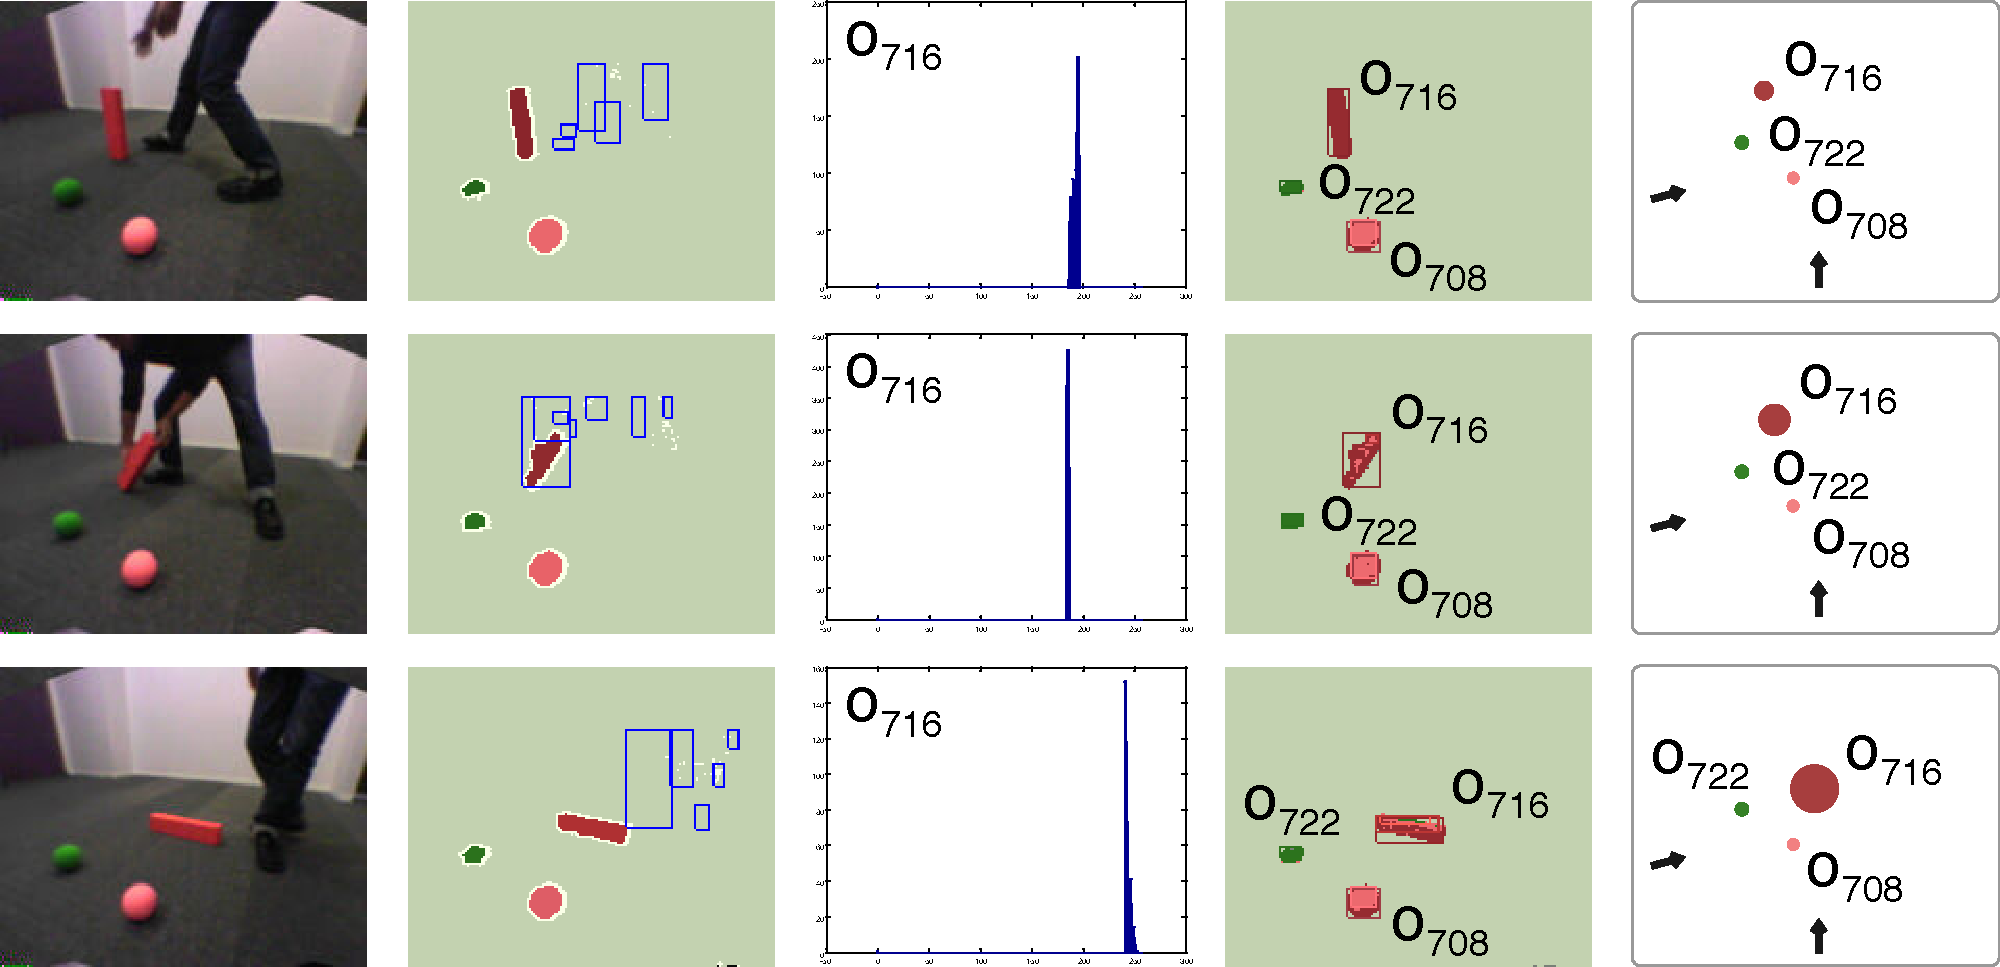
\includegraphics[width=.85\textwidth]{chap10/figs/png-perception.pdf}}
\caption{\label{fig:png-perception}A robot is looking at consecutive scenes (from top to bottom) and tracking the objects in the scene. One object (labelled $O_{716}$)
is moved by a human experimenter.  We see from left to right: the original source image, results of region detection and 
colour segmentation, the (average) value for one dimension of one object ($O_{716}$), the segmented and labelled objects, 
and the world model, including the position of the other robot (indicated by a pointing arrow). }
\end{figure}
\clearpage
We call the feature vector for each object a {\scshape sensory experience}. \is{sensory experience}
It is represented using a spiking 
diagram, with a spike for each dimension and the value on that dimension marked (see 
\figref{fig:prototypes-identifiers-words}, left-most column). Real
world vision is difficult enough, but because the robots look at the
scene from different points of view, they often do not carve out the
same regions and they will certainly see different views of the
objects and locate them in different positions within their own
egocentric reference frame. So sensory experiences of the same scene
are always going to be different. This makes coordination and hence successful
communication very challenging. 

Third, it is very difficult to establish which individual is associated with a particular
sensory experience because the appearance of an object changes, depending on
its posture, its position with respect to the viewer, and the changing
light conditions in the environment. A standard method in object
recognition, for which there is also evidence in human subjects, is to
capture the invariant properties of a particular view of an object in
terms of prototypes. A prototype has for each sensory dimension a typical value and a tolerated variance
within which the certainty of recognising the prototype decreases. Prototypes are also displayed using a spiking 
diagram, with a spike for each dimension and an indication of the best value as well as the minimum and maximum
(see \figref{fig:prototypes-identifiers-words}). Internally, agents store a set of cases 
and compute the mean value for each dimension as the typical value and the variance as a way to determine 
minimum and maximum cut-off points. So the learning and adjustment of categories is statistical in nature. 

The best matching prototype for a given sensory experience is \is{prototype} 
found by a weighted sum of the match for each dimension. Many neural network models exist that perform this kind
of computation, such as Radial Basis Function networks, and their behaviour is well
understood. But the difficulty here is that robots do not have access
to a clear data set of examples and counter examples from which they
can learn how a prototype should be defined. Moreover clusters found
through unsupervised learning (such as through Kohonen
nets) may not necessarily correspond to the prototypical
views of an object. In addition, each agent independently and autonomously
develops his own repertoire of prototypes based on his history of
interactions with the world and others. Hence it is totally unlikely
that the agents have exactly the same set of prototypes, which
further aggravates the coordination and communication problem. 

Fourth, although an individual may have some notion of the invariant properties
of an object, usually
there are significant differences between different views of the same
object. So reliable object recognition requires the acquisition of
different (prototypical) views and this raises the question how the
robots can know whether two quite different views (for example a front
view of an object standing up and a back view of the same object
laying down) belong to the same object. 

Finally, the robots must build up a lexicon associating names with individuals. When no name
exists yet, the robots can baptise the object with a newly invented name that
will spread in the population through consecutive games because
hearers can acquire the meaning of an unknown name based on feedback
from the speaker after a game. But since a language game is always a
local interaction between only two agents, it is possible that another
agent has invented a different name for the same object which also has
propagated to some extent, and so synonymy (different names for the
same object) is unavoidable. Moreover because of the inherent noise
and unreliability of visual perception and recognition of pointing
gestures as well as different prototype boundaries for different
agents, it is possible that one agent makes an incorrect guess about
the meaning of an unknown name or misinterprets feedback and thus
acquires a different meaning for a name. So homonymy (different
objects for the same name) is unavoidable as well. This raises the
critical question how a shared optimal vocabulary can be reached at
the level of the population without central control or telepathy,
which will require mechanisms for damping synonymy and homonymy at the
individual and population level.

\subsection{Semiotic networks}
We have already seen from earlier experiments that the solution to these various issues lies in setting up
the right kind of \dblenquote{semiotic dynamics}. In the present case, this dynamics should gradually coordinate
sensory experiences, prototypical views, individuals, 
and names, both within a single individual and across the
population. This led to the notion of a {\scshape semiotic network}, which was a significant conceptual advance 
in the methodology of conceiving and carrying out language game experiments.

\begin{figure}[b]
  \centerline{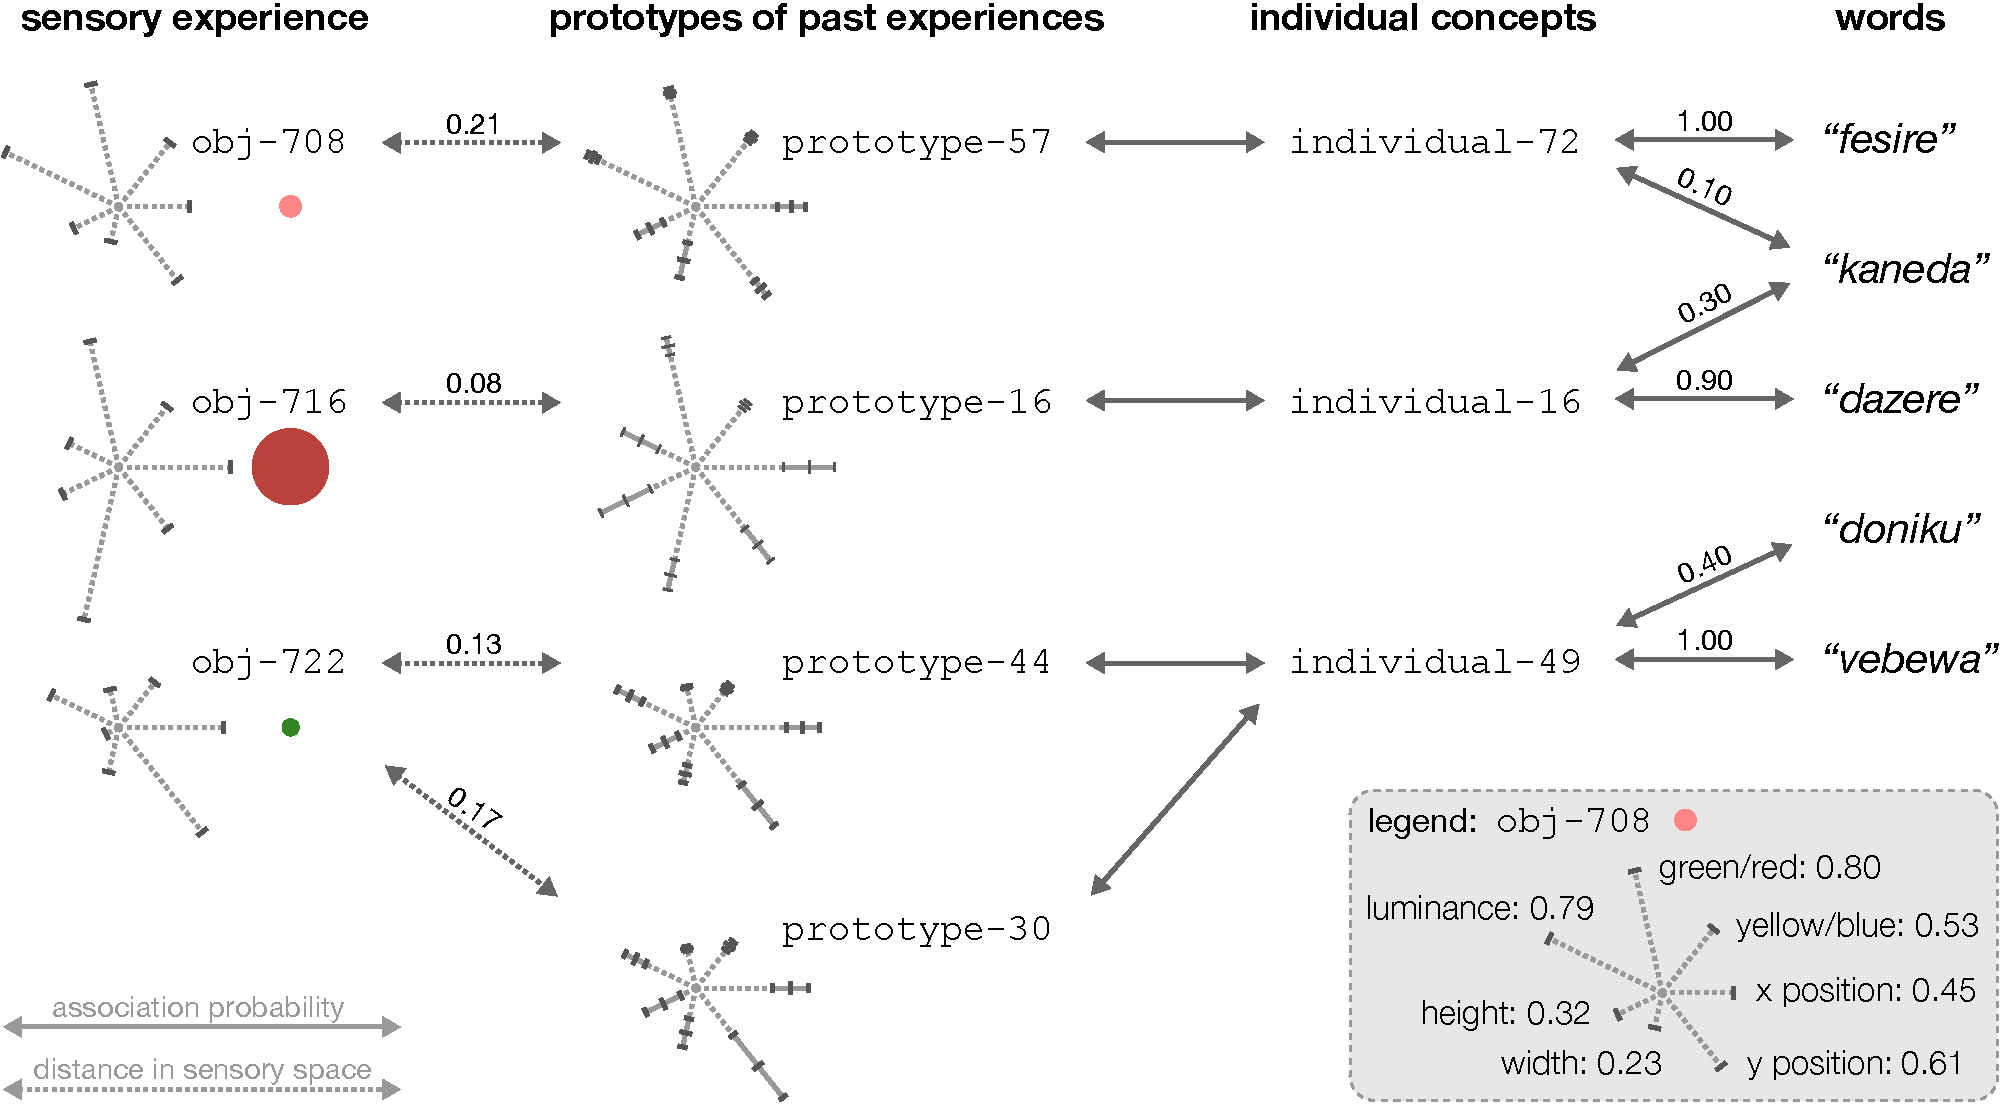
\includegraphics[width=.95\textwidth]{chap10/figs/prototypes-identifiers-words.pdf}}
\caption{\label{fig:prototypes-identifiers-words}In the Proper Naming Game experiment the memory of the agents is conceived in terms of a semiotic network that 
spans the full semiotic cycle from sensory experience and conceptualisation to naming.}
\end{figure}

A semiotic network of an agent $a$ is defined as 
${\cal S}_a = O_a \times V_a \times I_a \times N_a$ where $O_a$ is the set of
sensory experiences of the agent grouped per scene, $V_a$ the set of
prototypical views maintained by $a$, $I_a$ the set of individuals
 known to $a$, and $N_a$ the set of names in $a$'s vocabulary
(see \figref{fig:prototypes-identifiers-words}
). Each link in the network is weighted (with a real number between 0.0 and 1.0). The
weight of the link between a sensory experience and a prototypical
view is based on nearest neighbour computation. The other weights are
stored in memory and reflect the confidence of the agent in the use of
that link based on past experience. 

A semiotic network \is{semiotic network} is bidirectional and dynamic in the sense that new nodes can be added or
removed as a side effect of a language game and the weights between
nodes change based on the outcome of a game. In
order to decide which name to use for a chosen topic, the speaker
traces pathways in his private semiotic network. He starts from the
set of sensory experiences perceived in the current scene, activates
the best matching prototypical views, activates the individuals
linked to these prototypical views, and then looks up the names for
these objects. The pathway that has the highest cumulative score,
which is the sum of all weights of the links involved, is considered
to be the winner and the name occurring at the endpoint of this path
is the name transmitted by the speaker to the hearer. 

Conversely, in order to decide which physical object to point at given a name, the hearer
traces pathways in his own semiotic network but in the other
direction. He starts from the name, looks up the individuals
associated with this name, then the possible prototypical views
associated with this individual, and then the sensory
experiences belonging to the object regions in the current scene which
are the best matches with these prototypical views. The pathway with
the highest cumulative score is the winner and the object occurring at
the endpoint of that path is considered by the hearer to be the topic
to which he should point. The speaker then interprets the pointing
gesture and gives non-linguistic feedback about success or failure.

Given this notion of a network, the key question for designing an effective 
strategy for playing the language game becomes: What are the operators that are building and
changing the semiotic networks in each agent? We focus first on the
vocabulary, i.e. the links between nodes for individual objects $m_i$ and their 
names $f_i$. We use a variant of the strategy used in the Talking Heads experiment. 
Only the hearer changes the score after a game. 
In the case of a successful game, the score $\sigma_{f_i,m_i}$ of the used association is 
increased and its competitors are decreased according to the following
equations with the alignment rate $\gamma = 0.2$: 
\begin{equation}
 \sigma_{m_i,f_i} ≤\leftarrow \sigma_{m_i,f_i} (1-\gamma) + \gamma
\end{equation}
\begin{equation}
 \sigma_{m_j,f_i} ≤\leftarrow \sigma_{m_j,f_i} (1-\gamma) j \neq i
\end{equation}
\begin{equation}
 \sigma_{m_i,f_k} ≤\leftarrow \sigma_{m_i,f_k} (1-\gamma) k \neq i
\end{equation}
A competitor is another individual $m_j$ stored in the hearer's memory 
for the name $f_i$ or another name $f_k$ for the individual 
$m_i$. When the speaker is using a name which is not linked in the network 
of the hearer to any individual, then the hearer adds a new relation between 
the recognised individual (after pointing by the speaker) and this new name. 
This alternative then competes from 
now on with existing associations through the lateral inhibition dynamics. 
We already know from many other experiments that this strategy, when used collectively in 
consecutive games between randomly chosen members of the population, leads to the  
self-organisation of a shared lexicon due to positive feedback.\footnote{
The semiotic dynamics of lateral inhibition has been studied thoroughly by Bart de Vylder as reported in his Ph.D thesis 
(2007 at the VUB AI Lab) and summarised in this paper: \cite{deVylder:2006}.}
 
When an agent sees a scene in which there are different segments, each yielding their own sensory
experience, he can safely assume that these segments belong to 
different individuals and therefore must match best with 
different prototypes. If this condition is violated, the agent
can use the sensory experiences without a unique match as seeds for new
prototypical views and link them to newly introduced individuals.  
Prototypes are later adjusted to better reflect invariant properties by updating their 
mean value and variance. 


\begin{figure}[htbp]
  \centerline{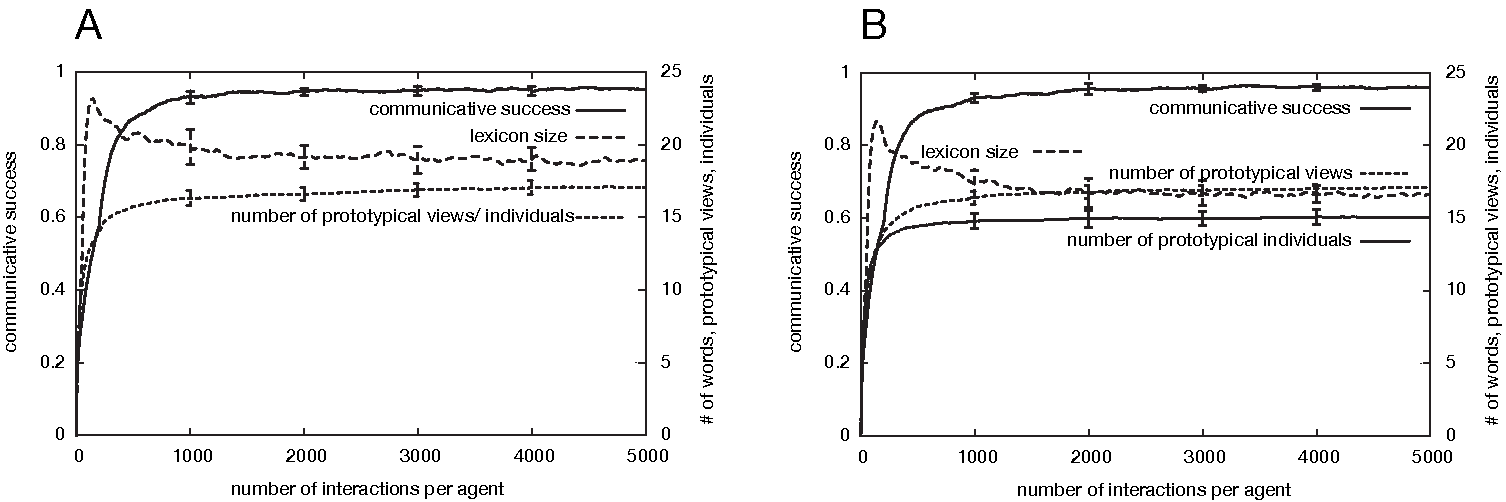
\includegraphics[width=\textwidth]{chap11/figs/png-results.pdf}}
\caption{\label{fig:png-results} 
{\itshape Left:} Results for Proper Naming games in a population of 10 agents that have to name 15 individual objects. 
We see that a vocabulary establishes
itself after agents have played a few hundred games. There is again the typical peak until alignment kicks in. 
The number of individuals is larger than 15, implying that agents name prototypical views rather than 
individuals. {\itshape Right:} Results after the addition  
of a heuristic based on tracking an object over time. We see that there are fewer individuals 
than stored prototypical views, which means that agents have improved their ability to recognise object 
identity. }
\end{figure}
With these mechanisms, the population reaches a high level of communicative success (above 90 \%). 
However the average number of individuals in the agents' semiotic networks
is much larger than the number of distinctive objects
introduced in the experiment (see \figref{fig:png-results}, left). Apparently, agents are naming prototypical views of
individual objects instead of the individuals themselves. So we did not adequately address 
how a robot learns to interrelate different views. To do this, various heuristics need to be added. 
\clearpage
We have operationalised just one example of such a heuristic. When an object is moving or being moved,
its appearance may change but the observer tracking the object 
still knows that he is dealing with the same object and so he can
exploit this information to fine-tune his semiotic networks. Because the vision system we used on the \textsc{qrio} robots, developed 
by Michael Spranger,\footnote{
This system is described in-depth in: \cite{Spranger:2012vision}.} is able to track an object, it can align object
regions across different images, enriched with top-down predictions of
how an object region will change over time based on Recursive Bayesian
estimation using Kalman filters. The object being moved by 
the experimenter in \figref{fig:png-perception} 
yields two quite different sensory experiences when standing up or lying down which match with 
two different prototypes, but thanks to the tracking heuristic, the semiotic network can 
be rearranged to reflect that they are two views of the same object (see \figref{fig:png-optimisation}). 


\begin{figure}[htbp]
  \centerline{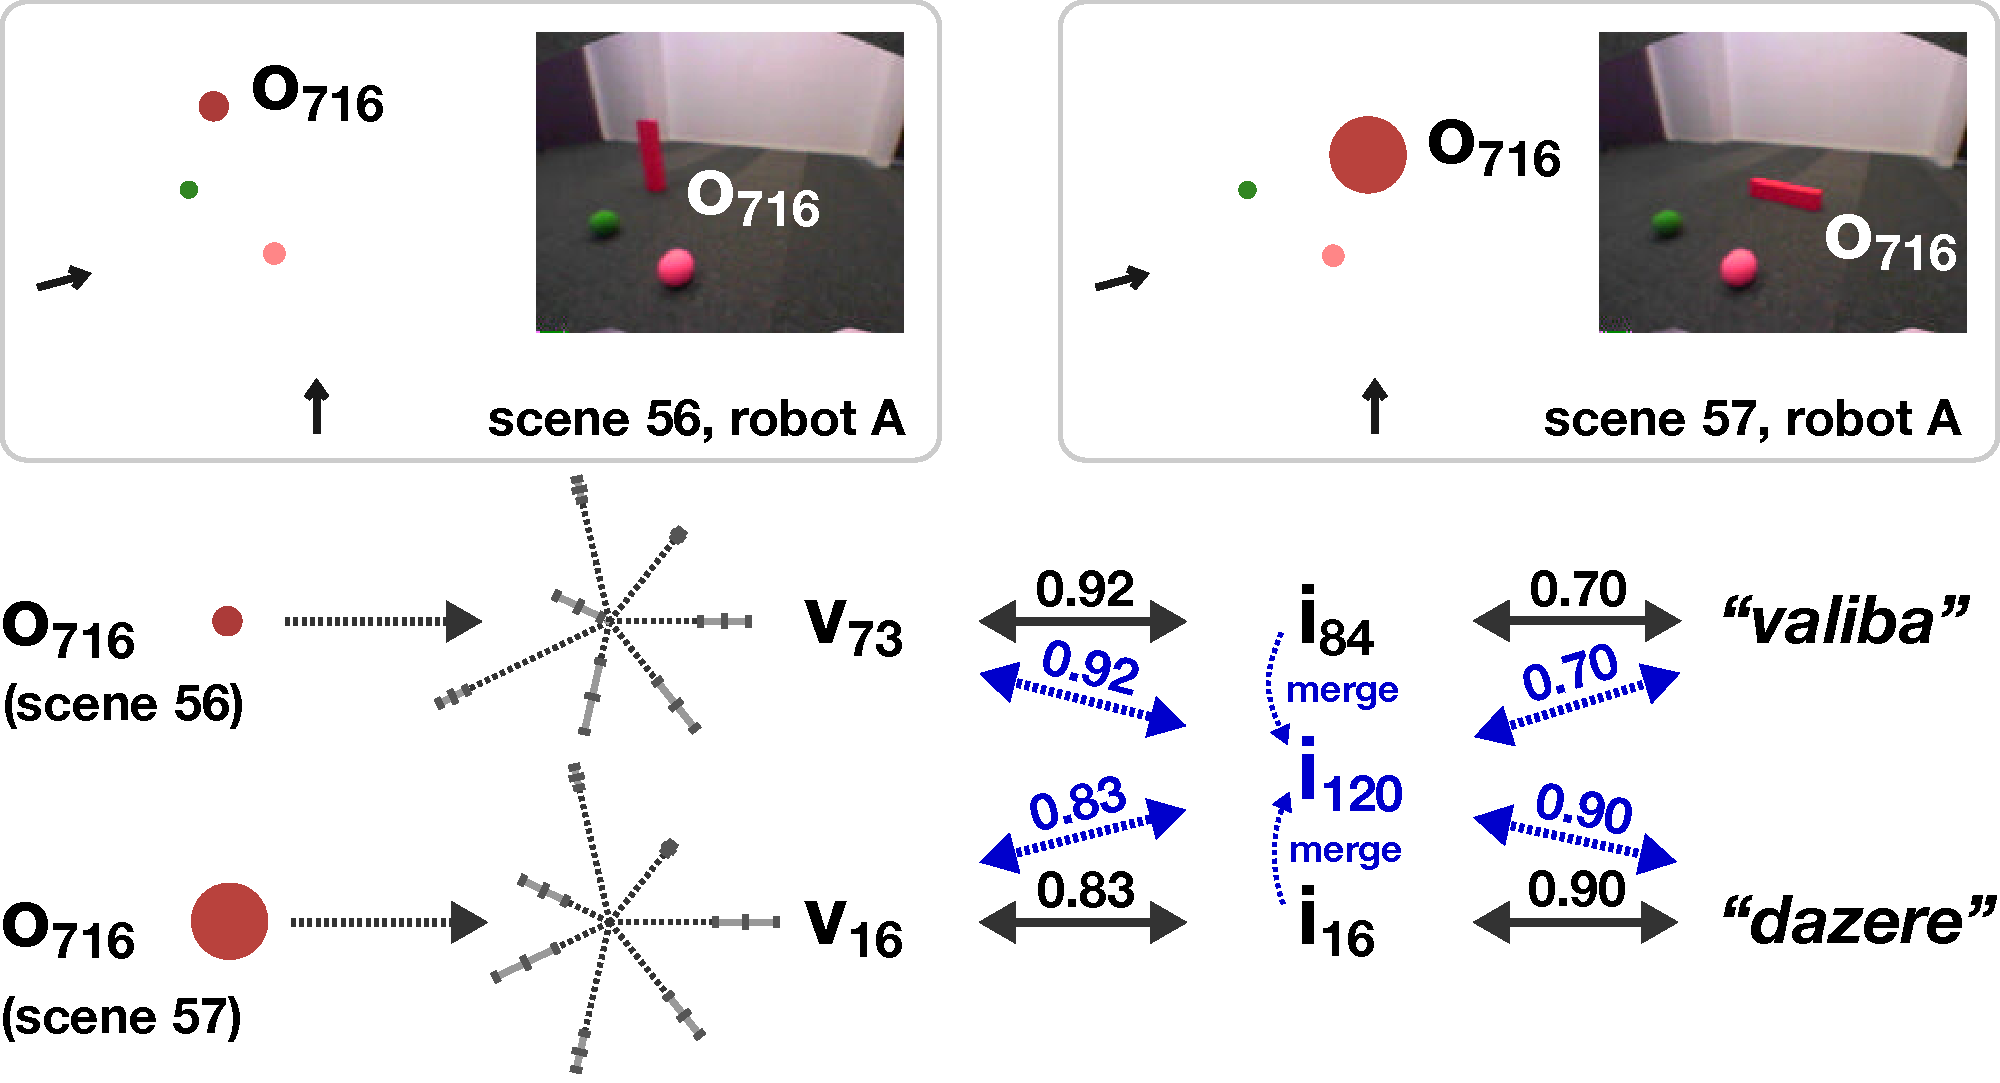
\includegraphics[width=.75\textwidth]{chap11/figs/adjust-id.pdf}}
\caption{\label{fig:png-optimisation}When the identity of two objects is discovered (because two prototypical views have been established 
as belonging to the same individual object), the former nodes for identities can be merged while keeping the 
links to their names intact. 
}
\end{figure}

\figref{fig:png-results}, right shows what happens when the robots use this heuristic. The population
exhibits still the same capacity to achieve communicative success as
in \figref{fig:png-results}, left, but now the number of individuals
has significantly lowered, becoming equal to the number of distinct objects 
that were introduced (i.e. 15). So the heuristic has done its work. 

Clearly humans use many additional heuristics. For example, if we see somebody walking into a
building with a refrigerator and we later see the same person on the
top floor handling a refrigerator we assume it is the same
refrigerator, even if we could not track this object. Or if we know that a particular person is 
going to come and visit, and next we hear the bell and open the door, we expect and recognise this particular 
person even if clothes or hair have changed drastically. The
point of the present experiment was not to operationalise all imaginable heuristics but to
show that heuristics help to optimise and coordinate semiotic
networks and thus further increase the ability of a population to develop internal shared
representations anchored in the world.

\section{Action Games} 

As a second example of how thinking in terms of semiotic networks is useful,
we turn to an experiment building further on the work on action-word learning \is{action game}
using the \textsc{aibo} reported in the previous chapter.
It was first designed and carried out with the \textsc{qrio} robot in 2007/2008 by Luc Steels and
Michael Spranger with considerable help from Martin Loetzsch\footnote{Papers describing this experiment more fully are: 
\cite{Steels:2008spatial} and \cite{Steels:2008b}.} and 
then ported in 2010 to the \textsc{myon}, a robot developed by Manfred Hild and his team at the Humboldt 
University in Berlin (see \figref{fig:myon-action}) (\cite{Steels:2012b}). 
A BBC video clip of the experiment can be seen at: \url{https://youtu.be/lmoXByLkK14}.
The porting exercise showed that once we discover how to do a certain type of language game on one robot 
we can relatively easily transfer it to another one, after adapting the lowest level sensing and actuation routines. 

\begin{figure}[htbp]
  \centerline{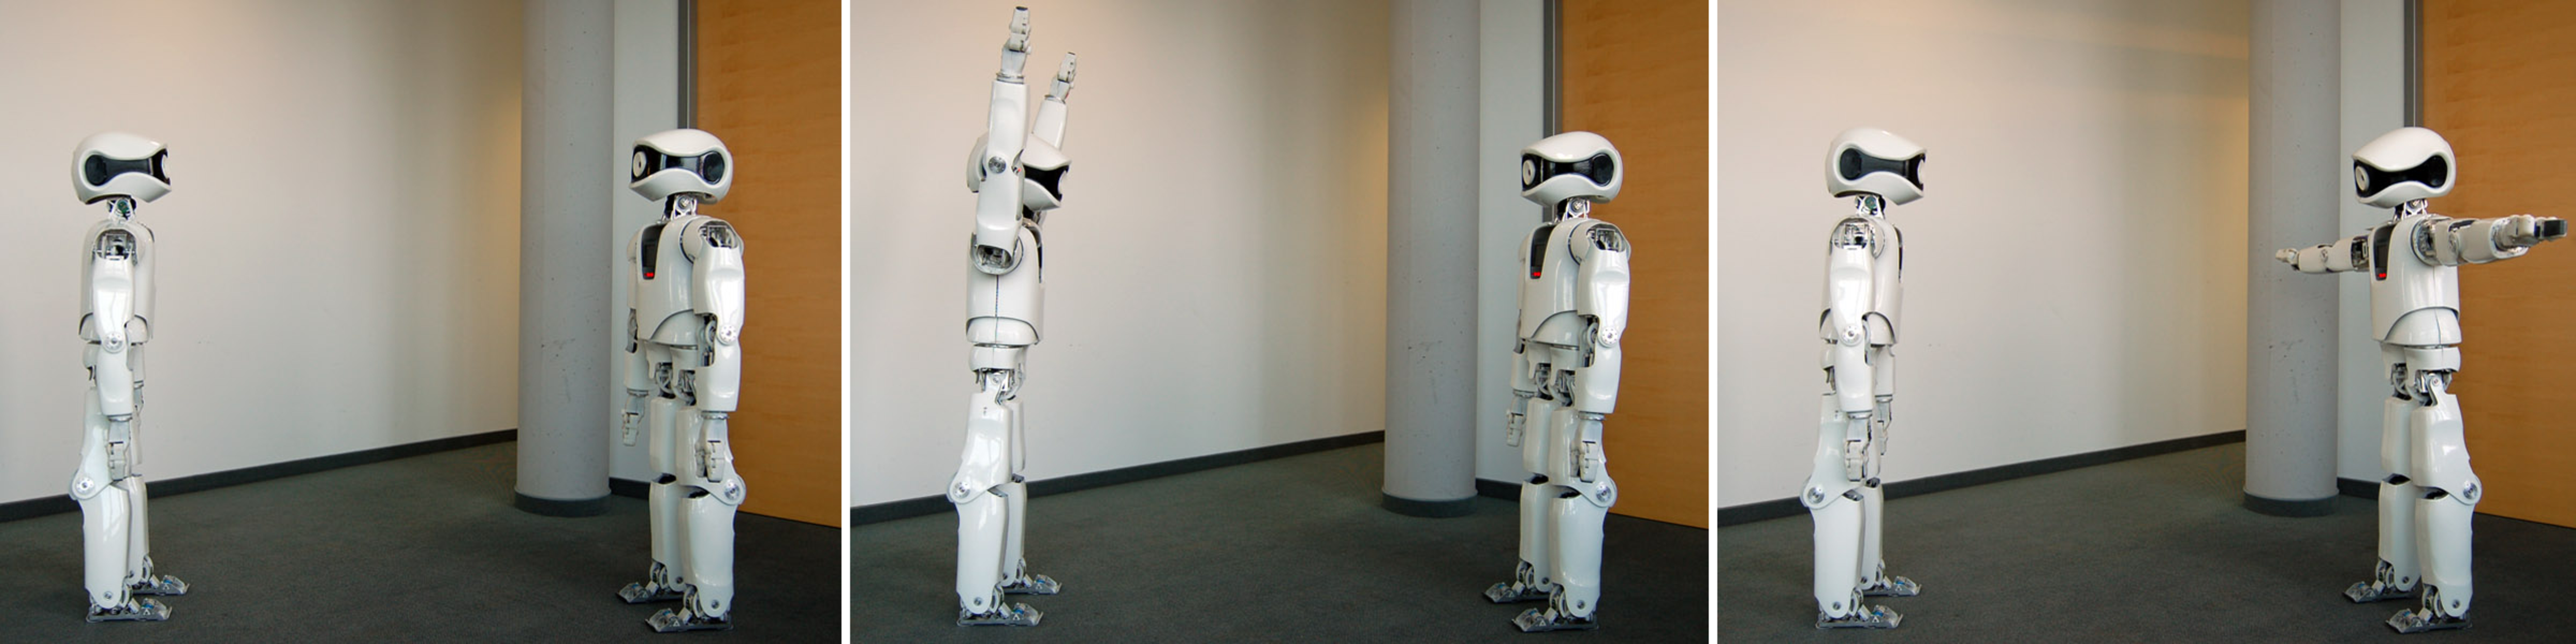
\includegraphics[width=1.0\textwidth]{chap11/figs/myon-action-game.pdf}}
\caption{
Two Myon robots playing an action game. One robot (the speaker) names an action and the other robot (the hearer) 
has to perform the action. When the hearer performs the right action the speaker signals success by nodding the head, 
otherwise he performs the action himself so that the hearer can adjust his semiotic network accordingly. {\itshape Left:} the speaker
requests an action. {\itshape Middle:} the hearer interprets this as moving up both arms. {\itshape Right:} correction by the speaker. 
}\label{fig:myon-action} 
\end{figure}

The basic goal of the experiment is to simulate the emergence of a repertoire of actions and action terms, such as 
\smplenquote{move up your left arm}, or \smplenquote{stretch out both arms}. As often, a seemingly straightforward semantic domain generates 
a set of fundamental subproblems that need to be solved and integrated so that the solutions work together: 

1. The robots need a {\scshape repertoire of actions}. So they need a sensori-motor system that allows them to carry out 
repeatedly and reliably an action. They can themselves observe the action both in the visual domain,  
looking at their own body or looking at their body in the mirror, or through proprioception, using sensors attached 
to the motors and joints on the body. There are many ways in which an action repertoire can be built up. One way 
is through motor babbling: The robot makes random movements and thus explores the sensori-motor 
space in order to find possible coherent actions. In the experiments reported here, the motor actions are acquired 
by kinesthetic learning: The experimenter moves parts of the body of the robot. These movements are recorded by the robot
and he can then play the movement back. 

2. The robots need to be able to recognise actions carried out by others. This can be accomplished again 
with a prototype-based approach, as in the Proper Naming Game described in the previous subsection. Each individual action 
is always slightly different from another instance of the same action and so totally accurate matching would not work. 
For example, two instances of the same \smplenquote{moving up both hands} gesture will always look slightly different because of the 
position of the hands and arms and the exact starting body posture of the robots or the perspective from which 
the gesture is perceived. 

The features used in the experiment focus on the upper torso of the robot and are based on a binary 
version of the original image. They rely on a standard pattern recognition technique, known as Normalised 
Centralised Moments (\cite{Hu:1962}). \is{Normalised Centralised Moments}
Moments are a global description of shape, capturing the statistical regularities
of its pixels for area, centre of mass, and orientation. Centralised moments are invariant to translation and 
normalised moments are invariant to translation and scale. Here we use seven moments, so that an image schema of 
the upper torso is captured in terms of a feature vector with seven data points, represented as a graph, 
although it could also be represented using the spike diagram used in the Proper Naming Game (\figref{vision}, right). 
These feature vectors are then classified using the same prototype-based approach as in the Proper Naming Game. A prototype of a posture 
consists of typical points for the seven moments, as well as a minimum and maximum deviation from 
each point. The best matching prototype is found by nearest neighbour computation. New prototypes are created 
when there is no prototype that matches distinctively with the sensory experience of a body posture and matching prototypes are
slightly adjusted to integrate new instances, so that the prototype progressively and adaptively reflects the body postures observed
in the world. 

3. The robots need a {\itshape mirror system} that relates perceived actions carried out by others to their own actions. 
The topic of mirror systems has received a lot of attention the past decade because cells were discovered in the brain 
that serve this purpose.\footnote{
An overview of mirror system research and its relevance to the question of the origins of language is given here: 
\cite{Rizzolatti:1998}.}
However the fact that such cells are discovered in the brain 
does not yet tell us how mirror systems are being learned or how they operate. For the action language game, we tried 
several approaches.

\enlargethispage{1\baselineskip}
In one of them, the robot stands before the mirror (\figref{robot-mirror}) and observes its own 
postures, which generates the data for learning the association between body postures and prototypes. 
The robot selects a posture, and activates the corresponding motor behaviour. This motor behaviour generates a sensory image and 
hence a sensory experience categorised with a particular prototype. Through standard Hebbian learning (which enforces the 
connection between nodes that are simultaneously active) the link between the posture prototype and the motor action gets 
established and progressively enforced. 
\clearpage
\begin{figure}[p]
\centerline{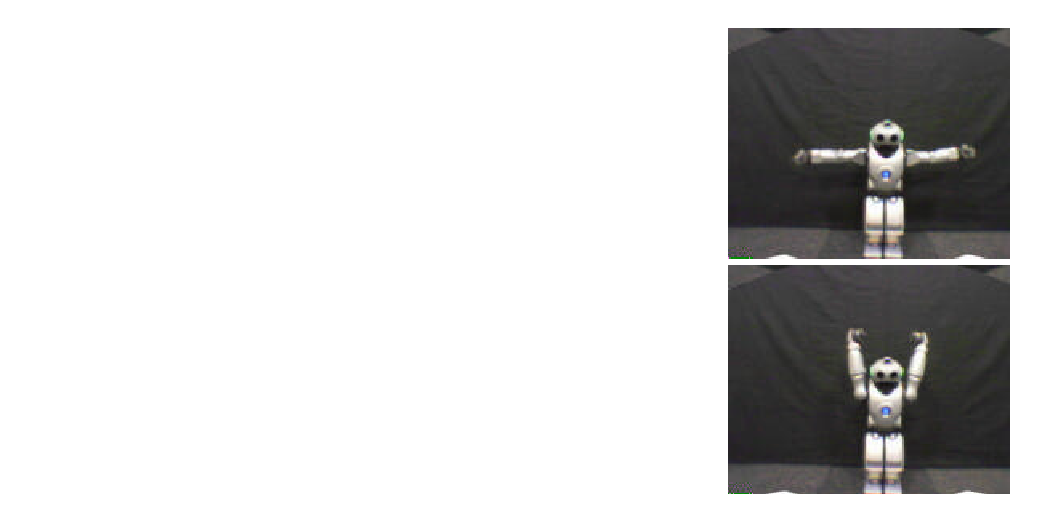
\includegraphics[width=0.2\linewidth]{chap11/figs/postures.pdf}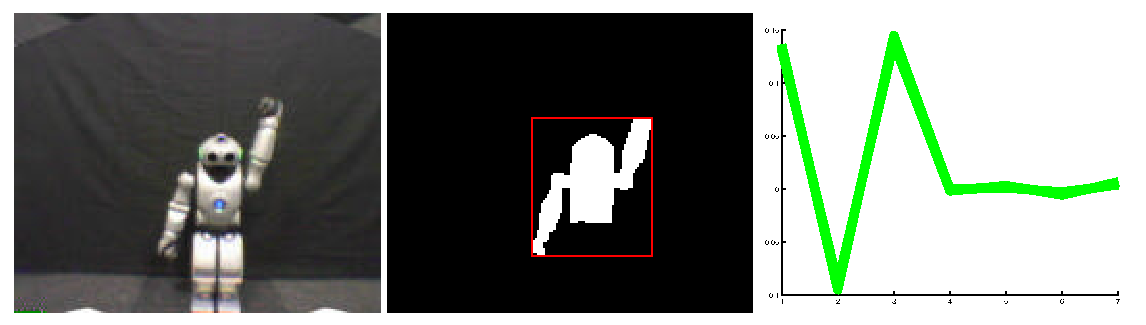
\includegraphics[width=0.75\linewidth]{chap11/figs/vision_2.pdf}}
\caption{\label{vision}{\itshape Left:} Example postures of the robot (which is the \textsc{qrio} in this case).
{\itshape Right:} Visual analysis. From left to right we see the source image, the foreground/background distinction and object segmentation (focusing on the upper torso), and the feature signature of this posture represented as a graph connecting the values (on the y-axis)
of the seven centralised normalised moments (on the x-axis).}
\end{figure}

\begin{figure}[p]
\centerline{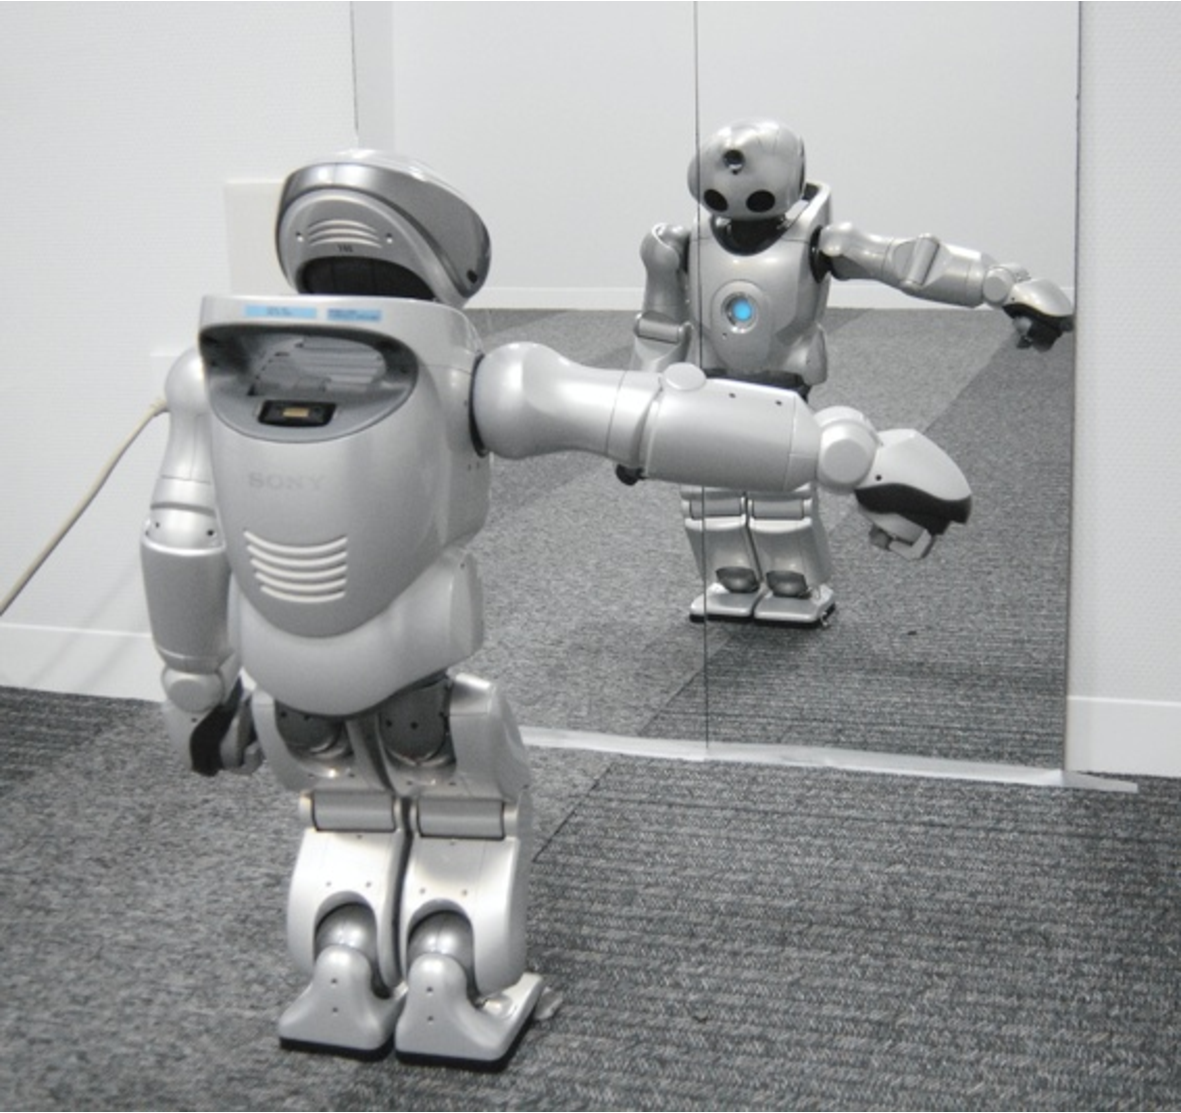
\includegraphics[width=0.6\linewidth]{chap11/figs/robot-mirror.pdf}}
\caption{\label{robot-mirror}The \textsc{qrio} humanoid robot stands before a mirror and performs various motor behaviours thus observing what visual body-images these behaviours generate.}
\end{figure}

Because all robots have the same body shape, a robot can use visual posture prototypes of 
himself in order to categorise the body image of another robot, after 
perspective reversal. Perspective reversal means that the robot is able to detect the position of the other 
robot and is able to perform a geometric transformation to map the visual image of the other robot onto 
the canonical body position of itself.

4. Once the robots have a reliable mapping between image schemata of postures and body movements, the 
lateral inhibition dynamics used in the Proper Naming Game can easily solve the task of evolving 
a shared vocabulary. The score of the association between a word and a posture prototype is increased in a successful 
game and synonyms decreased. In an unsuccessful game, the score of the used association is decreased. 
\figref{commsuccess} 
shows the global behaviour of a population of 10 agents after each individual has coordinated motor 
behaviour and visual body-image through the mirror for 10 postures. 100 \% success is reached easily after about 
2000 games. After 1000 games, which means 200 games/agent, there is already more than 90 \% success. 
The graph shows the typical overshoot of the lexicon in the early stage 
as new words are invented in a distributed fashion followed by a phase 
of alignment as the agents converge on an optimal lexicon. 


\begin{figure}
\centerline{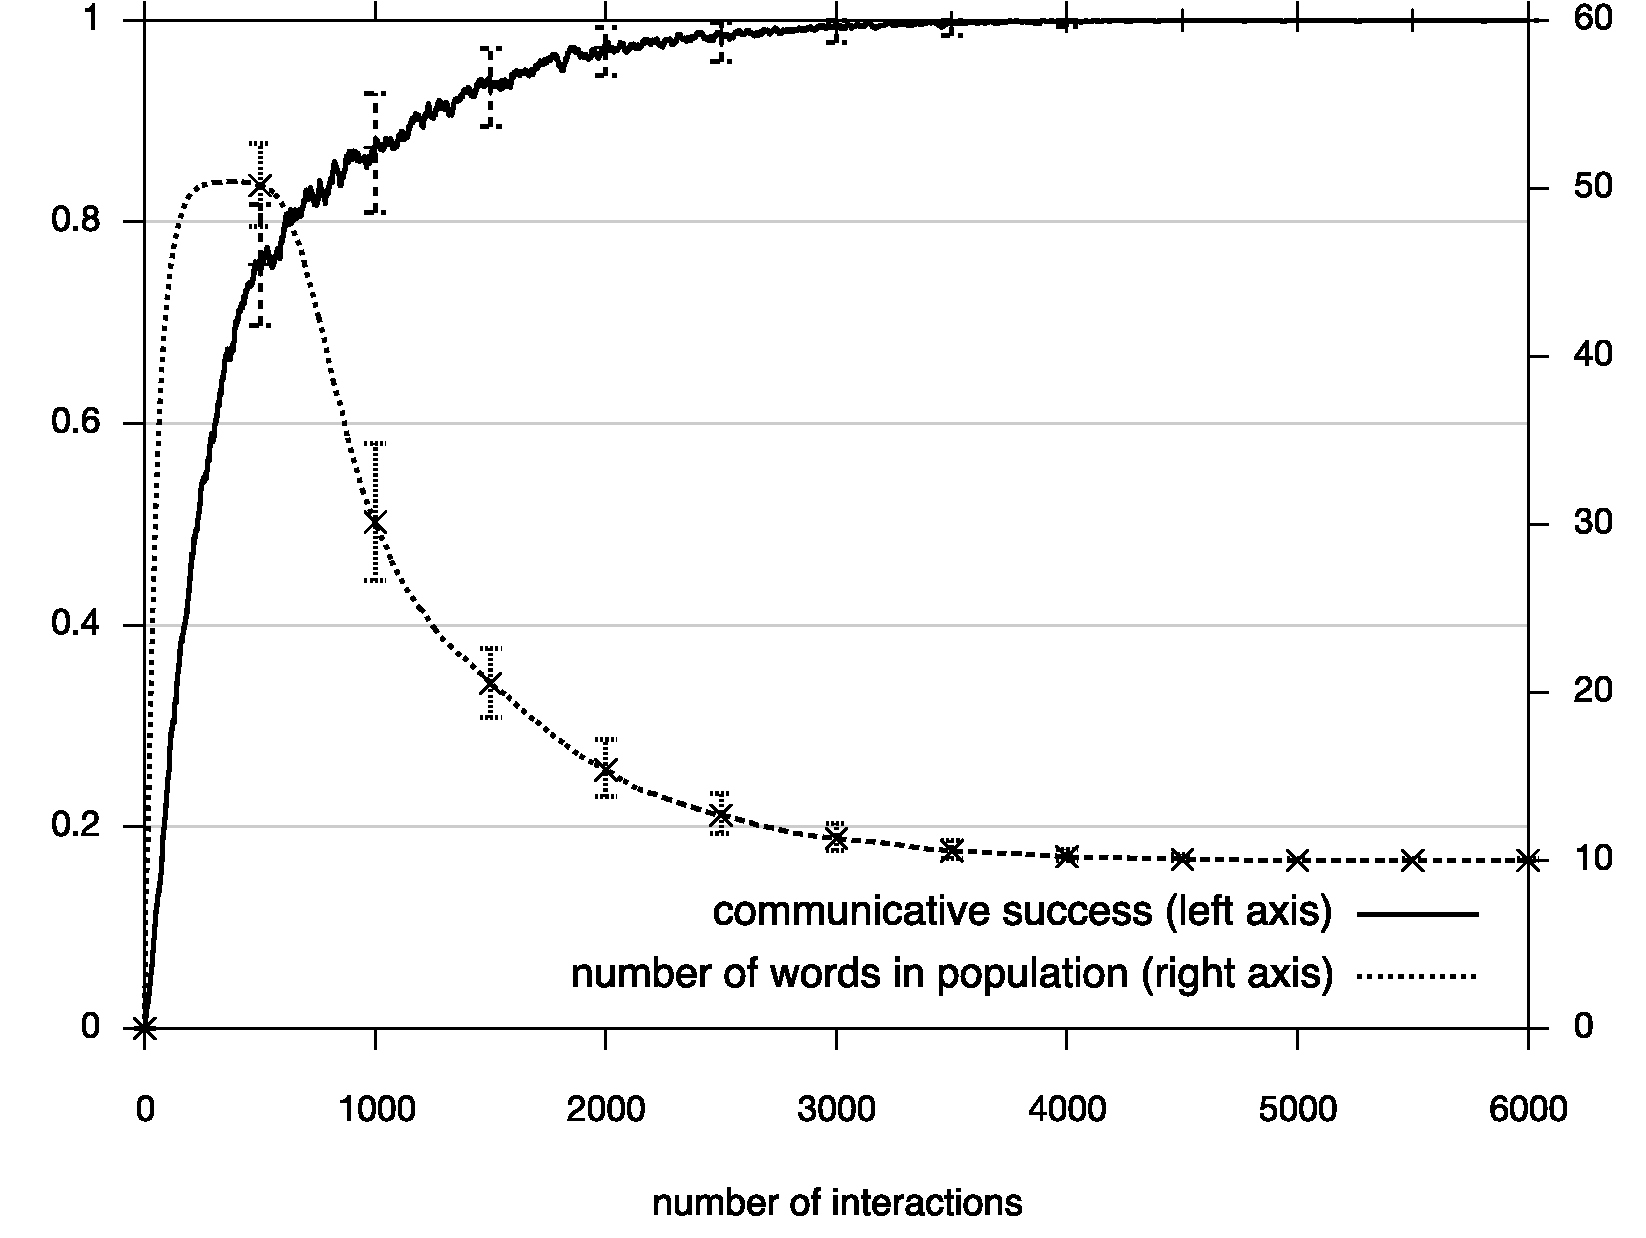
\includegraphics[width=0.6\linewidth]{chap11/figs/commsuccess.pdf}}
\caption{\label{commsuccess}Results of the Action Game played by a population of 10 agents 
for 10 postures after coordinating image schemata and motor control through a mirror. 
The x-axis plots the number of language games. The y-axis shows the running average of 
communicative success and average lexicon size.}
\end{figure}

This experiment shows that other language games, which do not rely on feedback through pointing, can be set up easily. 
Here the feedback happens through the actions of the hearer. The experiment also shows
that the same technique of setting up a semiotic network can be applied to other domains. 
The network used here is shown in \figref{network}. Compared to the Proper Naming Game, we see the same relation between 
sensory experiences, visual prototypes, postures (instead of nodes for individuals), 
and words. But now there is an extra dimension because motor behaviours 
achieving a posture are also linked with the posture nodes. This suggests also another approach besides the use of a mirror 
for coordinating the relationships between perception and motor action: When the hearer has learned to associate a word with a particular
posture node through the visual prototype of this posture, he can later get feedback on which motor behaviour should be 
associated with the same posture node, or, vice-versa, he can first learn the association between a motor behaviour and 
a word (when the speaker asks to perform the posture) and then learn what visual prototype corresponds to that. 
Experiments show that this method indeed also works to achieve a coherent mirror system, \cite{Steels:2008}.


\begin{figure}
\centerline{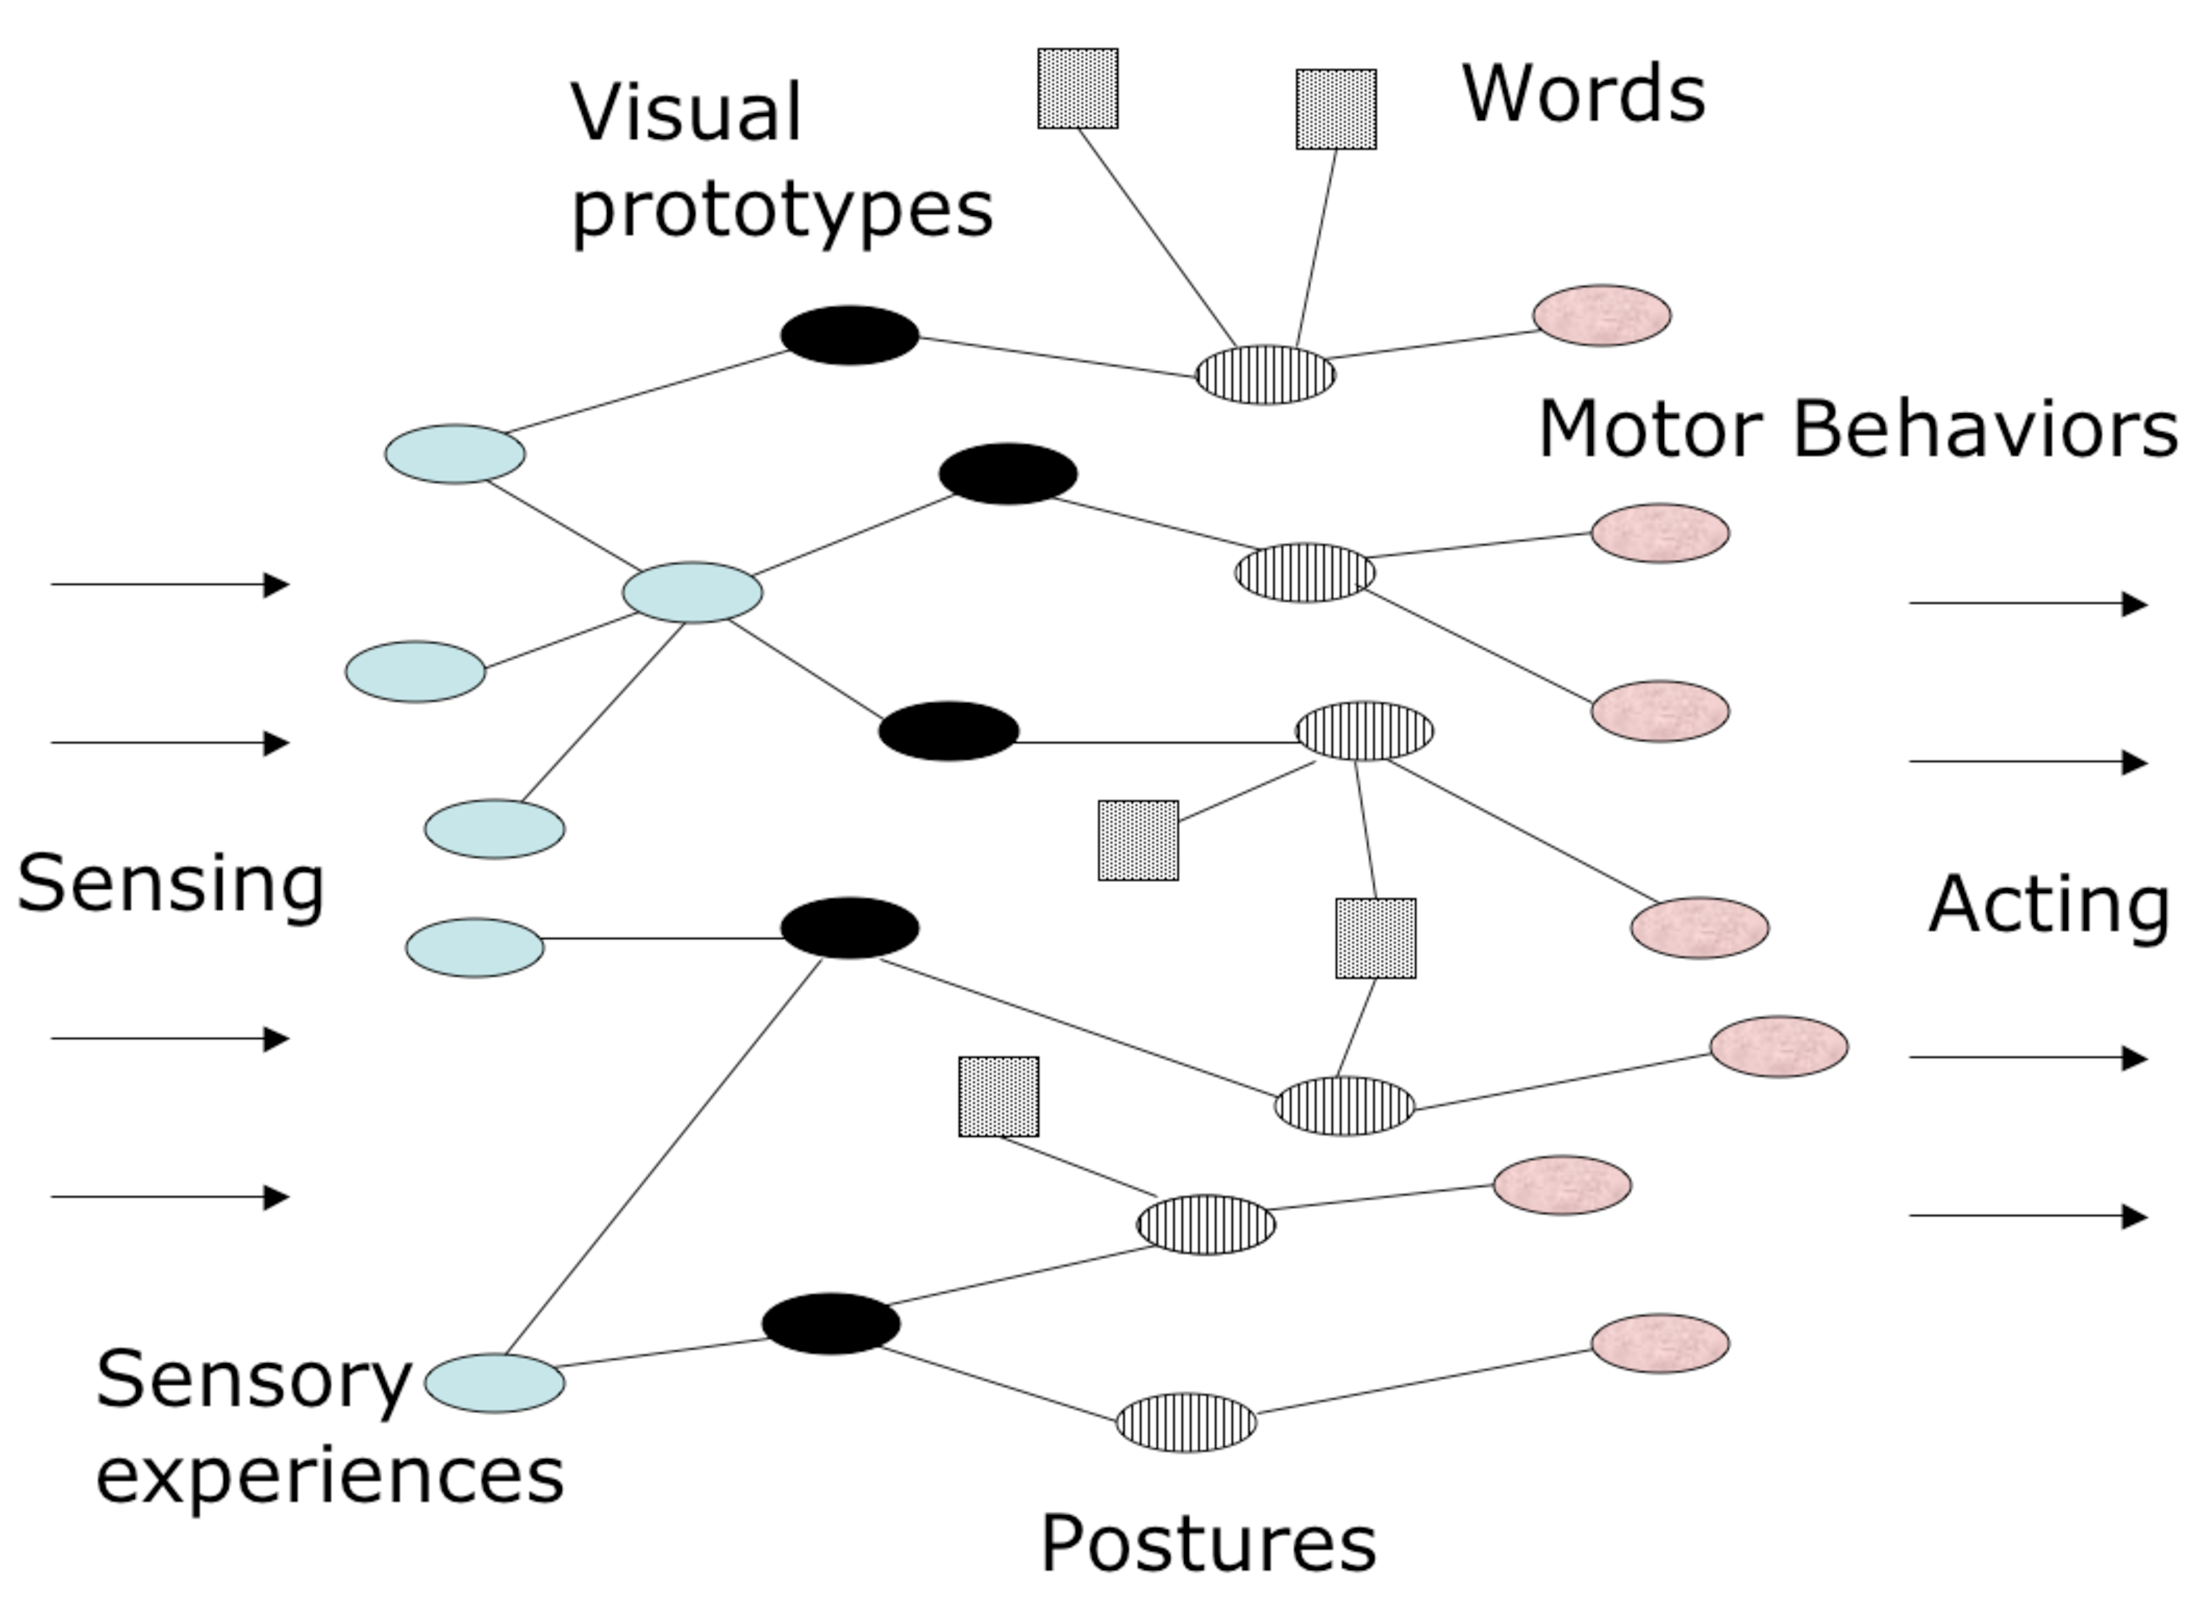
\includegraphics[width=0.6\linewidth]{chap11/figs/network.pdf}}
\caption{\label{network} Semiotic network linking sensory experiences, visual prototypes of postures, nodes for postures acting as mirror neurons, and nodes triggering the motor behaviour that achieves the posture. Nodes for words (shown as squares) 
are associated with the posture nodes.}
\end{figure}

\section{The Colour Description Game}

Already from 2001, as a direct follow up of the Talking Heads experiment, in-depth experiments were started on the emergence of 
colour vocabularies. This topic was chosen because 
there is a substantial body of research on colour in the cognitive sciences, with 
detailed analysis of its underlying biology, psychological experiments on colour perception and categorisation 
and extensive work, often building further on the studies of Berlin and Kay, on colour language. It is also 
relatively easy to carry out colour naming game experiments, because it does not require complex feature extraction 
and pattern recognition. Moreover the grammar for colour descriptions is highly restricted and so it is a good micro-domain for 
advancing not only research in the interaction between categorisation and naming but also in grammar. 
\is{Colour Description Game}

In our group, Tony Belpaeme became the main Ph.D researcher for Colour Naming, finishing his thesis 
in 2005.\footnote{The first extensive paper on this research appeared as: \cite{Steels:2005}.}
This work was then continued by Joris Bleys, who managed to scale up from colour naming to colour description with 
a thesis defended in 2010.\footnote{This thesis is published as another volume in the present series as: \cite{Bleys:2014}}
The colour domain has attracted several other language game researchers, attempting to explain 
universal trends in colour categorisation.\footnote{Most notably: \cite{Puglisi:2008}, \cite{Baronchelli:2010}.}


\begin{figure}[htbp]
  \centerline{\includegraphics[width=.65\textwidth]{chap11/figs/color-qrio.pdf}}
\caption{\label{fig:munsell}Set-up with two \textsc{qrio} humanoids, similar to Munsell chip tests used in psychology. The same game as the Talking 
Heads was used, but only colour chips were provided as input and the robots use pointing and head movements to 
provide feedback.}
\end{figure}

When the \textsc{qrio} humanoid robots became available, we decided to use this existing work for pushing forward the state of 
the art in colour language research in two ways:
\begin{itemize}
\item To use more realistic circumstances of object perception. Because 
robots are moving around in three dimensions and see the situation from different points of view, the reflection 
of light changes and is different for speaker and hearer (see \tabref{f:scene-example}). This difference did not 
play a role in earlier experiments but 
it certainly plays an important role in the stabilisation and choice of colour prototypes. 
\item To focus on colour descriptions beyond basic colour terms, i.e. descriptions like 
\textit{slightly blue}, \textit{blue-green}, \textit{bluish green}, \textit{very bright}, \textit{shiny yellow}, \textit{dark red}, \textit{sky blue}, 
\textit{very dark bluish red}, etc. Indeed, it turns out that 
basic colour terms are used only in about 10 to 15 \% of the occurrences of colour descriptions. The rest are 
more complex expressions. Complex colour descriptions require scaling up the semantics and introducing grammar, they 
also require the introduction of language strategies as a layer of abstraction 
above lexical and grammatical constructions. 
\end{itemize}


\begin{table}[htbp]
  \centering\small
\begin{tabular}{ccc}
 \lsptoprule 

    &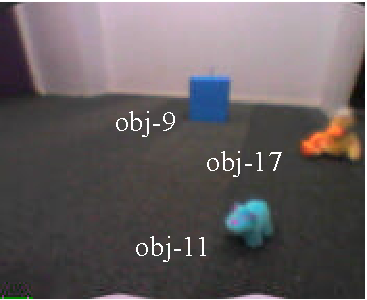
\includegraphics[width=0.37\textwidth]{chap11/figs/grounding-scene-a.pdf}
	&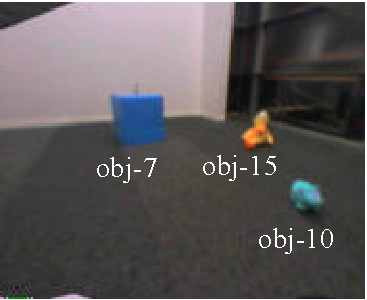
\includegraphics[width=0.37\textwidth]{chap11/figs/grounding-scene-b.pdf}\\
  \multicolumn{2}{c}{
    \begin{tabular}{lrrr}
	      & obj-9 & obj-11 & obj-17 \\
    \midrule
    \emph{L*} &  35.5 &  51.2 & 50.5 \\
    \emph{a*} &   7.7 & -17.1 & 26.7 \\
    \emph{b*} & -40.7 & -14.0 & 39.6 \\
    \end{tabular}
  }
&
  \begin{tabular}{rrr}
 obj-7 & obj-10 & obj-15 \\
\midrule
      35.6 & 52.8 & 62.2 \\
      7.2 & -20.1 & 27.9 \\
      -39.0 & -11.3 & 52.5 \\ 
  \end{tabular} \\
\lspbottomrule
\end{tabular}
  \caption[Comparison between the colour perceptions of two robots for
  an example scene]{Colour perceptions of two
    robots for the same scene. The robots see the yellow duck
    (obj-17 for the left robot and obj-15 for the right robot) from
    different sides and distances and thus perceive very different colour values on 
    the \emph{a*} and \emph{b*} colour dimensions for the same object.}
  \label{f:scene-example}
\end{table}

Together with Joris Bleys and using the vision system developed by Michael Spranger, we 
performed language game experiments both for the same set-up as shown in \figref{fig:grounded}, 
i.e. geometric objects in an environment but now ignoring all dimensions except those related to colour, 
and from a set-up that was similar to the Munsell chips used
in psychological experiments (see \figref{fig:munsell}). The colour space used by the agents was the CIE L*a*b* space, where 
L stands for lightness and a* and b* are the two opponent channel dimensions (yellow-blue and red-green). 

A language strategy has two components: (i) a particular way of conceptualising reality (and learning the categories involved
in this conceptualisation) and (ii) a particular grammatical pattern that suggests to the listener what strategy is intended 
and provides the contents to execute the strategy. For example, in the phrase \textit{very green}, the combination of an adverb 
\textit{very} and a basic colour adjective \textit{green} suggests a \dblenquote{graded membership strategy} where not only a basic colour prototype
(\textit{green}) is introduced but also how close the sample is to this prototype (\textit{very}). I will now introduce first how 
the conceptual aspect of a language strategy is defined using a procedural semantics system called IRL and then how the 
linguistic aspect is defined, using Fluid Construction Grammar. 

\subsection{Compositional procedural semantics with IRL}
% {\bfshape Compositional Procedural Semantics with IRL}\\

Procedural semantics, dating back to research on natural language understanding in the 
early seventies by Philip Johnson-Laird, Terry Winograd and Bill Woods, argues that the meaning of an utterance is 
equal to a program.\footnote{See for the early research in particular: \cite{Winograd:1971}, \cite{Woods:1981}, 
\cite{Johnson-Laird:1977}.} \is{procedural semantics}
This approach is very amenable to grounded language understanding, because programs can be physical 
actions that the robot executes or operations over the internal states in memory, such as retrieving information
from the visual data, performing perspective reversal, storing information, etc. Procedural semantics
contrasts with a logic-based approach to semantics which assumes that facts are available in a fact base and semantics operates
by matching queries against this database. The problem for a logic-based approach
is that there is an infinite amount of
information that can be computed about the world and so it is not possible to get a 
complete set of facts. Instead, language actively constrains what facts are collected about the world. For example, if 
we say "the red ball", the hearer knows that he has to focus on the shape and colour of the objects in front of him, 
and so attention and processing resources can be targeted to those feature dimensions. 

To work out the procedural semantics hypothesis, we need to address the question what the primitives are of 
these semantic programs, and what computational formalism is most suited to combine them. Already in 2000, I reported
a representation system for computational semantics, called IRL.\footnote{
The earliest paper introducing IRL is: \cite{Steels:2000}. 
A more recent description of a new implementation is reported as: \cite{Spranger:2012}.}
IRL stands for Incremental Recruitment Language, for reasons that will become clear soon. \is{IRL}
IRL uses a constraint language approach. Constraint programming languages were pioneered in the  \is{Constraint Programming}
seventies by Borning, Steele, and others. It is a very active field with its own conferences, 
organisations and journals\footnote{see \url{http://www.informatik.uni-trier.de/ley/db/journals/constraints/}.} 
with wide applications in user interfaces, scheduling problems, design, games, etc. 

The basic idea of a constraint language is that only data flow is expressed explicitly, not control flow. 
There is a set of slots (variables) and a constraint attempts to reduce the set of possible 
fillers (bindings) for a slot. Constraints are combined in 
a constraint network, based on sharing slots. A solution is found when every slot in the network has unique bindings. 
Usually it requires looping several times through the constraints and often even a rewiring of the constraints to 
find a solution. A numerical example of a set of constraints on natural numbers could be:
\begin{verbatim}
  x = y + z with 2<y<5 and 0<x<5
\end{verbatim}
The constraints expressed here form a network because the same variables x and y (which are the slots of the 
network) appear in different constraints (the sum constraint and two instances of the <-constraint). 
Given this network, constraint propagation can compute easily that x = 4, y = 3, and z = 1. 

\enlargethispage{2\baselineskip}
IRL formalises constraints using prefix notation in the following way. Slots are symbols preceded 
by question marks. Constraints are defined with a list with the first argument the name of the constraint and 
the remaining arguments the slots: 
\begin{verbatim}
 (<constraint> <arg1> ... <arg-n>)
\end{verbatim}
The first argument is called the target of the constraint because it is the most logical ``outcome" 
of applying a constraint, but as shown in the example above, data may flow in all directions. The numerical 
example given earlier translates into the following IRL program. 
\begin{verbatim}
(sum ?x ?y ?z)
(between ?y 2 5)
(between ?x 0 5)
\end{verbatim}

How are constraints defined? We need to specify for every possible case how the constraint can help to 
constrain the possible values of its slots. 
Just focusing on the sum constraint, we have the following cases:
\begin{itemize}
\item If ?x and ?y are filled (i.e. bound) 
we can compute ?z by ?z = ?x - ?y. 
\item If ?y and ?z are filled we can compute ?x by ?x = ?y + ?z. 
\item If ?x and ?z are filled we can compute ?y by ?y = ?z - ?x. 
\item If all three are filled we can test whether the constraint relation holds. 
\item If only ?x or ?y or ?z is filled, then it is not really possible to compute any of the others directly, but we can start 
to enumerate all possibilities if this is a finite set. 
\end{itemize}
The latter is not always possible because any number from the infinite set of numbers can be a filler 
and so it is better to wait until 
perhaps other constraints are able to limit the set of possibilities further. But for finite domains 
it might be conceivable to generate a set of possibilities. Concretely, for the above example  
the between-constraint could easily generate the list of possible numbers between the two given values.

IRL is a general language for defining constraints and constraint networks. The IRL system includes a 
constraint engine (which propagates constraints) as well as a constraint network planner, which finds a possible 
constraint network, given available information and a goal. Because a constraint network is a structure, it 
can also be matched against other constraint networks, for example, to complete a partial network or to find a network 
that is similar to another one. 

Constraint networks are an obvious choice for grounded (natural) language processing. \is{constraint network}
For example, to interpret the sentence \textit{the ball behind
the block}, it is possible that there are many blocks, many balls, but only one ball that is behind a block. So the 
unique referent of \textit{the ball}, \textit{the block} and of the total noun phrase only become clear when 
all constraints have been applied. Natural languages clearly do not supply control information but assume that 
the interpreter is smart enough to interpret constraints based on data flow. The other properties of constraint 
programming are also important. The constraint network planner can be used for conceptualising what to say and 
the constraint network matcher is highly useful in parsing an incomplete language fragment or in learning the 
meaning of a new grammatical construction.

\subsection{Building blocks for natural language semantics}
% {\bfshape Building Blocks for Natural Language Semantics }\\

What is the nature of the constraints that we will need for the semantics of natural language? 
Take a phrase like \textit{the ball behind the block}. It invokes the following constraints, also called 
semantic operations: 
\begin{itemize}
\item \textit{the ball} evokes a constraint to use a prototype [\textsc{ball}] to find a referent in the current scene.
\item The same holds for \textit{the block} which uses another prototype [\textsc{block}]. 
\item The preposition \textit{behind} implies another constraint, namely to use the spatial relation [\textsc{behind}] to filter a 
set of objects (namely those found by using the [\textsc{ball}] prototype) and retain only those that satisfy the behind-relation 
to an object in another set. 
\end{itemize} 

In IRL notation we get the following. There are first variables for the semantic entities (prototypes and relations) 
involved:
\begin{verbatim}
(bind prototype ?prototype-1 [BALL])
(bind prototype ?prototype-2 [BLOCK])
(bind relation ?relation-1 [BEHIND])
\end{verbatim}
Next there are four constraints: to get the context, come up with the set of blocks
(bound to ?object-set-1), the set of balls (bound to ?object-set-2), and then pick out the object 
that is a member of both sets and satisfies the behind-relation (bound to ?referent): 
\begin{verbatim}
(get-context ?context)
(filter-using-prototype 
   ?object-set-1 ?prototype-1 ?context)
(filter-using-prototype 
   ?object-set-2 ?prototype-2 ?context)
(select-object-using-relation ?referent ?object-set-1
   ?object-set-2 ?relation-1)
\end{verbatim}
Note how the different semantic operations are linked together because they share slots.
?referent is the final result of the network, which would be the topic of the language game. 

It should be possible for the filter-using-prototype operation
to either apply a filler for ?prototype-1 and 
?context and then compute ?object-set-1, or provide ?object-set-1 and ?context and obtain a filler for ?prototype-1. 
The 'normal' use is the first one, but the second use is just as important in planning what to
say (as speaker) or in guessing a possible prototype while learning the meaning of some unknown word. 
Moreover the \dblenquote{identify-set-using-prototype} operation can be made smart enough that it can actually come up with
a new prototype, when there isn't one yet that does the job. Hence learning can be 
integrated directly into the constraint network itself. 

So IRL is in fact a way to integrate the broad set of mechanisms used in 
pattern recognition (including neural networks) and AI (including machine learning). 
For example, an operation could implement a radial-basis-function network for doing categorisation and 
use the network to identify an object in a set. It could not only use the network but also adapt 
the weights in the network. Another operation could implement categorisation based 
on discrimination trees (as discussed in \chapref{chap:4}) and would not only do it, but also expand the discrimination trees 
when necessary. Other operations could implement set-theoretic operations, 
for the semantics of connectives like {\itshape and}, {\itshape or}, and {\itshape not}, by carrying out
{\scshape union}, {\scshape intersection} and {\scshape complement} operations over sets. There is no 
limit to the possible semantic operations, except that they have to terminate in finite time, possibly giving up when 
they cannot reach a valid result. IRL just provides a framework to define these operations and make them available 
to be recruited by the constraint network planner. IRL uses LISP as the host language, which means that all 
the computational machinery of LISP is available to implement semantic operations and associated learning algorithms. 

The constraint network planner works on an evolutionary basis, similar to genetic algorithms. Starting from the goal 
(for example identifying a particular object in the environment), it will generate possible networks by recruiting 
existing primitive operations, linking them in, and checking whether the computation makes progress towards reaching the goal. 
The slots of a constraint are typed to limit what semantic operations will be tried next. Networks that perform useful 
functions are \dblenquote{chunked} into higher order units that then can be used as units in their own right, thus scaling up 
complexity. These chunked networks become associated with stereotyped grammatical expression, so that there is a very 
fast retrieval and semantic execution.
\subsection{Strategies for colour}
% {\bfshape Strategies for Colour} \\

Let us now look at concrete examples from the colour domain as worked out by Joris Bleys, studying the following 
strategies: \is{colour strategies}

\enlargethispage{1\baselineskip}
1. The first strategy is the {\scshape Basic Colour Strategy} which implements a prototype-based approach to 
the basic colour categories. This approach is similar to the one used in the Proper Naming Game, except that 
only the three colour-dimensions are profiled (the opponent channels red-green, yellow-blue and the brightness channel). 
The strategy is similar to the one shown earlier. 
\begin{verbatim}
(equal-to-context ?s1) 
(profile-colour-dimensions ?s2 ?s1)
(filter-by-colour-lenient ?s3 ?s2 ?cc)
(select-most-activated ?t ?s3)
\end{verbatim}
When the speaker says \textit{green}, this network is used together with a specific binding of ?cc to the prototype for 
green (denoted as [green]). 
\begin{verbatim}
(bind colour-category ?cc [green])
\end{verbatim}
A graphical representation of this network is shown in \figref{fig:basic-strat}. 

\begin{figure}[htbp]
  \centerline{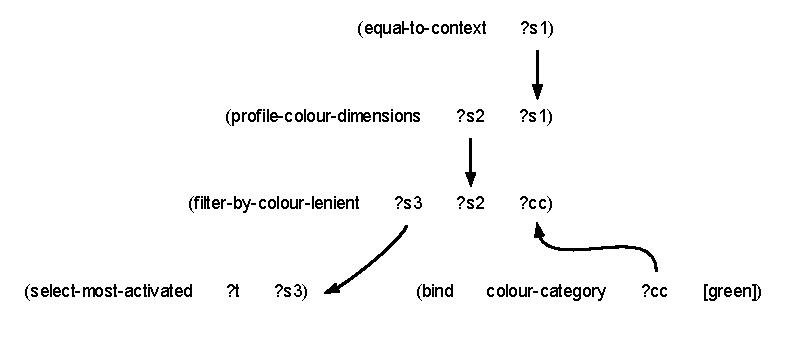
\includegraphics[width=1.0\textwidth]{chap11/figs/basic-strat.pdf}}
\caption{\label{fig:basic-strat}Constraint network for the Basic Colour strategy. The colours of each object in the context are retrieved, their 
similarity to the prototype computed, and the one with the highest similarity is chosen.}
\end{figure}

2. The second strategy is the {\scshape Graded Membership Strategy} which categorises the topic first using 
a basic colour but then qualifies how well its colour fits with the prototype. For example, we can say \textit{greenish} or
\textit{very green}. Some languages (such as Tarahumara spoken in Northern Mexico) obligatory mark graded membership using 
suffixes. The core of the constraint network is defined as follows. A graphical representation of the network is shown
in \figref{fig:graded}. 
\begin{verbatim}
(equal-to-context ?s1) 
(profile-colour-dimensions ?s2 ?s1)
(filter-by-colour ?s3 ?s2 ?cc)
(filter-by-membership ?s4 ?s3 ?mc)
(select-most-activated ?t ?s4)
\end{verbatim}
This network grabs the objects in the context and binds them to ?s1 using the equal-to-context operation. 
The profile-colour-dimensions operation picks out the colour properties of the various objects in ?s1 resulting in 
a new set ?s2. The filter-by-colour operation computes for each object in the set ?s2
how well they match with the prototype bound to ?cc, constructing a new set ?s3. The filter-by-membership operation 
then computes how well 
each object in ?s3 satisfies the graded membership qualification bound to ?mc, 
constructing ?s4. And then the select-most-activated operation picks out the best candidate and binds it to ?t. 
Other data flows within the same network are possible, for example to find the bindings of ?mc and ?cc given 
a context and a referent ?t that needs to be identified. 


\begin{figure}[htbp]
  \centerline{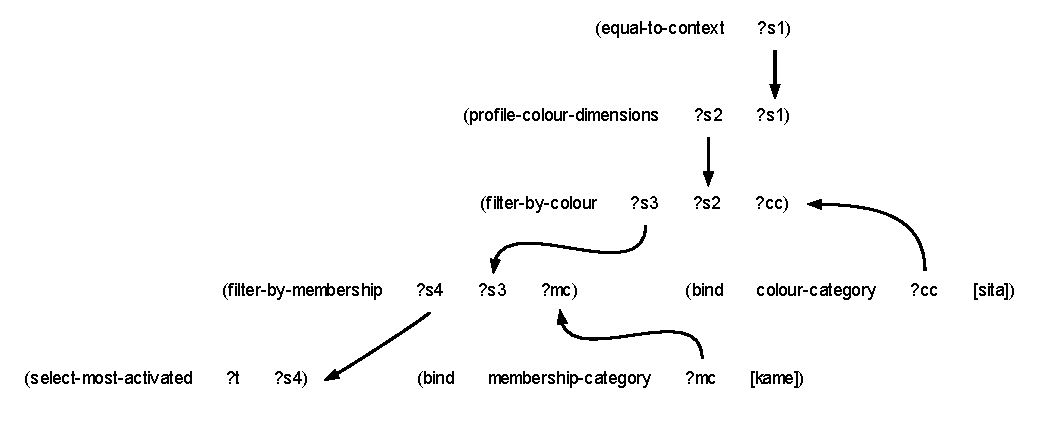
\includegraphics[width=1.0\textwidth]{chap11/figs/graded.pdf}}
\caption{\label{fig:graded}Constraint network implementing the Graded Membership Strategy. It builds further on the network for Basic Colour
Categorisation but adds a constraint to handle graded membership. }
\end{figure}
\enlargethispage{1\baselineskip}
The network is entirely general for all expressions that use graded membership and gets instantiated for a particular 
case by specifying the semantic entities involved using the bind operation. For example, Tarahumara has the word 
\textit{sita} for a particular colour prototype and \textit{kame} for one type of graded membership: 
\begin{verbatim}
(bind colour-category ?cc [sita])
(bind membership-category ?mc [kame]) 
\end{verbatim}

3. The third strategy is the {\scshape Category Combination Strategy} which compounds a category into two new ones, in 
expressions like \textit{greenish blue} or \textit{red orange}. This compounding is not a simple intersection. The set of objects  
that are \textit{greenish blue} is not found by taking all the ones that are green and all the ones that are blue and then 
the intersection of the two. Rather, it appears that the discretisation of the colour landscape is scaled with respect 
to the colour which appears as head of the phrase and then categorisation is done. This is achieved with the IRL network 
shown in \figref{fig:combi}. 
%http://www.workwithcolour.com/red-orange-colour-hue-range-01.htm

\begin{figure}[htbp]
  \centerline{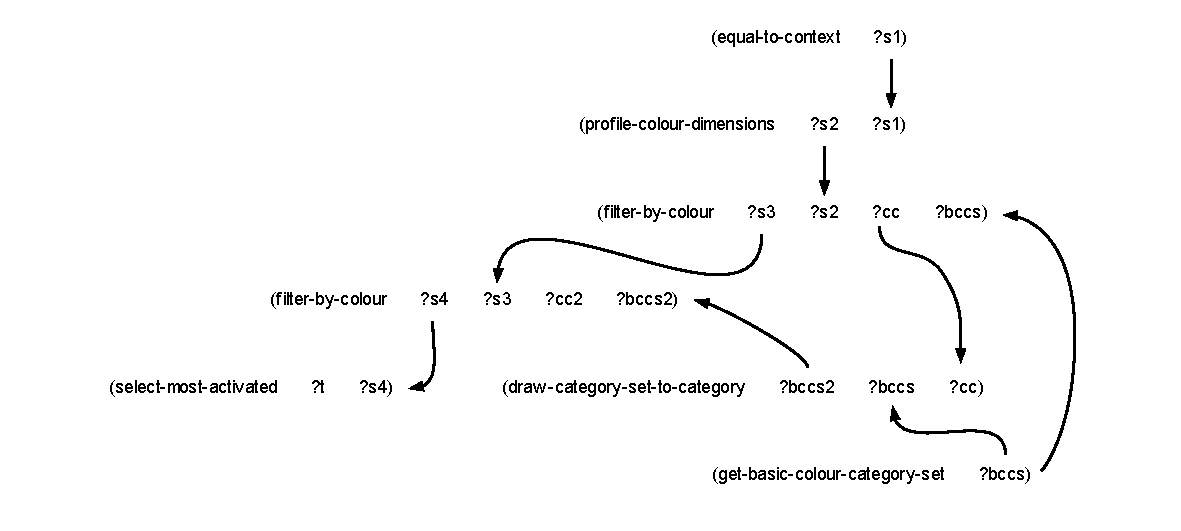
\includegraphics[width=1.0\textwidth]{chap11/figs/combi.pdf}}
\caption{\label{fig:combi}Constraint network implementing the Colour Combination strategy leading to expressions like \textit{greenish blue}. 
The filter-by-colour operation now has an extra argument, namely category-sets,  
and there is a draw-category-set-to-category operation that rescales the basic colour category set.}
\end{figure}

4. The next strategy is the {\scshape Basic Modification Strategy} which modifies a colour along the brightness dimension, as in 
\textit{light green}, \textit{dull yellow}, etc. It is implemented by projecting the modifying dimension onto the basic colour space 
whereby the colour being modified lies on the projecting vector and a new discretisation of the colour space can be 
performed. The network for this strategy is shown in \figref{fig:modi}. 
%http://www.workwithcolour.com/red-orange-colour-hue-range-01.htm

\begin{figure}[htbp]
  \centerline{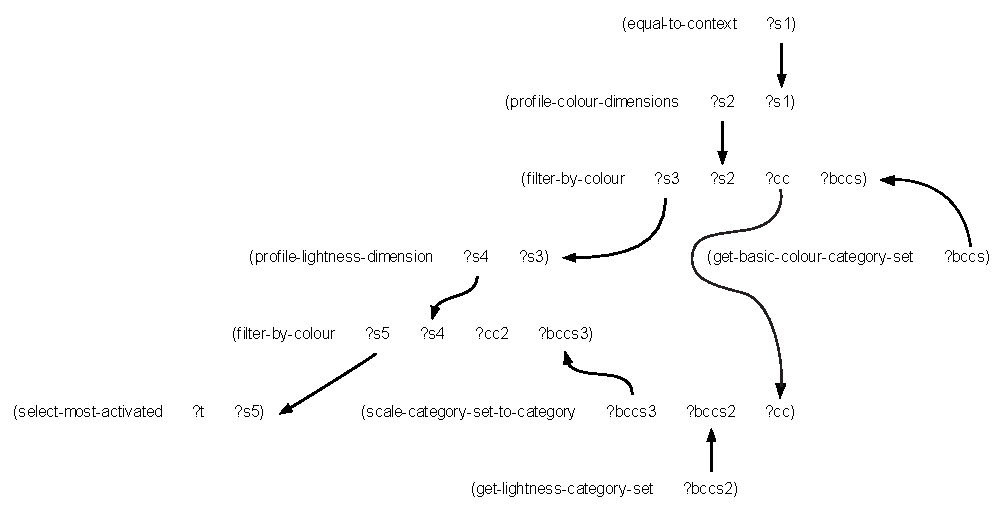
\includegraphics[width=1.0\textwidth]{chap11/figs/modi.pdf}}
\caption{\label{fig:modi}Constraint network for the basic modification strategy, for expressions like \textit{light green}.}
\end{figure}

Many other strategies for colour can be imagined and some of them are found in human languages (although not necessarily in English). 
These strategies always involve operations over the colour space (such as rescaling, dimensionality reduction, etc.) alongside 
additional operations (such as getting the context, picking out a referent, computing the intersection of two sets, etc.).

\subsection{Translation to grammar}
% {\bfshape Translation to Grammar} \\

The Colour Description Game used the Fluid Construction Grammar (FCG) formalism which was meanwhile being developed by our 
group with the explicit aim of supporting experiments in language emergence and evolution. A full exposition of this 
formalism falls outside the scope of the present book, but there is now a considerable literature for the interested 
reader (\cite{Steels:2011}). Here we just look briefly at the basic principles by which IRL 
expressions are translated into utterances. 

FCG represents syntactic and semantic structure in terms of units which have a set of features and values for these 
features. The features can be about any layer of linguistic analysis, from phonetics and morphology to various 
forms of syntactic description (constituent structure, functional structure, argument structure, information structure), 
semantic categorisations or meaning. 
The syntactic structure to express the basic colour strategy involves three levels of hierarchy. Units are built 
and expanded by three types of constructions (see for example \figref{fig:syntactic-graded}, left, which is an instantiation of 
the Basic Colour strategy in \figref{fig:basic-strat}). 

1. There are first {\scshape lexical constructions} that associate a word with the introduction of a semantic entity  
such as a colour category or a qualifier for indicating graded membership. So the meaning for the word \textit{yellow} 
introduces a \textsc{bind}-operation, as in: 
\begin{verbatim}
((bind colour-category ?c [yellow]))
\end{verbatim}
When the word \textit{yellow} is encountered, a unit for this word is created with this \textsc{bind}-operation as meaning and the 
word-string itself as the form. It is the unit called Yellow-unit in \figref{fig:syntactic-graded}. 
The construction also introduces a lexical category (part of speech) for the word (in this case the lexical category 
is colour-category) and specifies which variables in the meaning can be linked with other variables in other
units. The variables are typed. In this case there is one variable ?c which is of type colour-category. 

\begin{figure}[htbp]
  \centerline{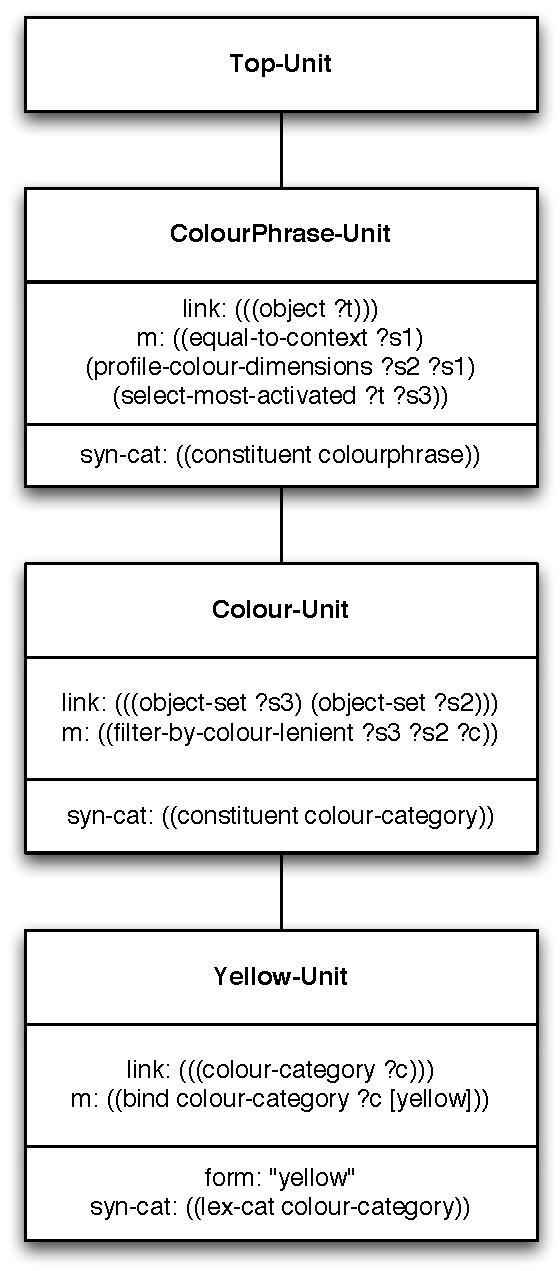
\includegraphics[width=0.3\textwidth]{chap11/figs/syntactic-basic.pdf} ~~~~ 
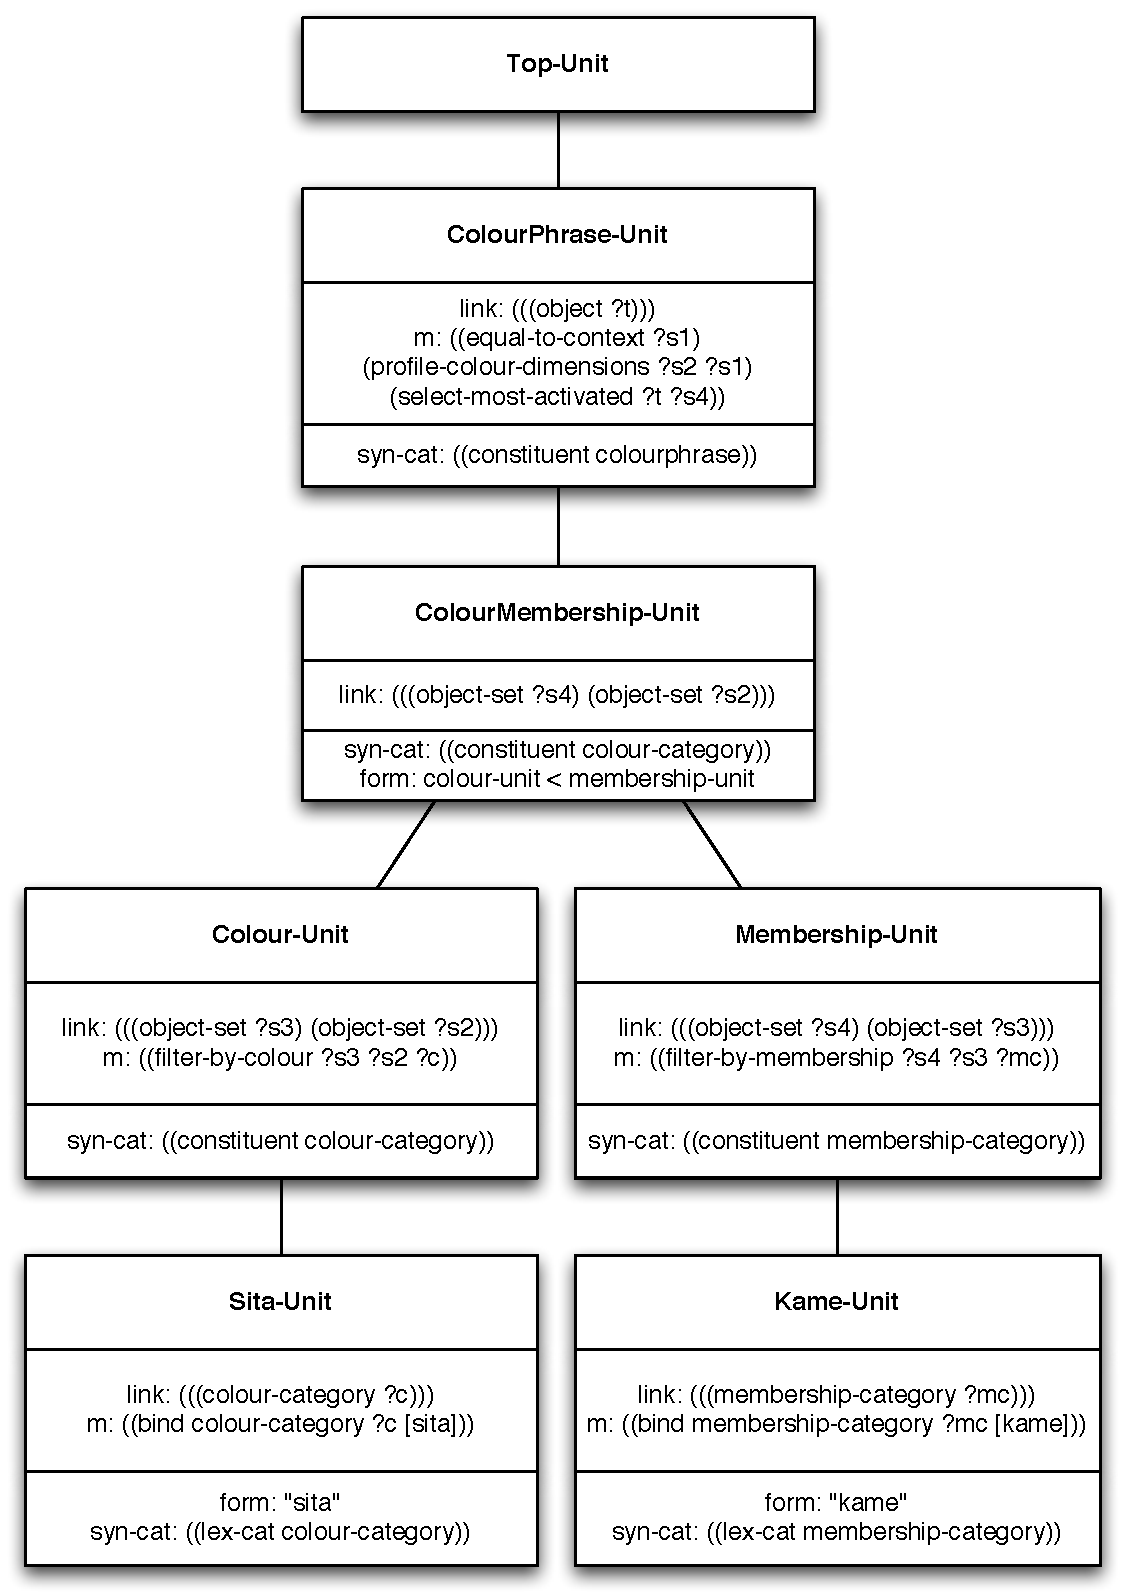
\includegraphics[width=0.6\textwidth]{chap11/figs/syntactic-graded.pdf}}
\caption{\label{fig:syntactic-graded} 
{\itshape Left:} Example of structure for the Basic Colour strategy. It involves three levels of hierarchy: for the word 
itself, the function of the word, and the combination of the different functions into a Colour-Phrase. Each box 
shows the name of the unit, and some of the key features of the syntactic and semantic pole.
{\itshape Right:} Example of structure for the graded colour strategy.}
\end{figure}

2. Next there are {\scshape functional constructions} that determine in which semantic operation the meaning of a word 
will play a role. It is necessary to have this layer above lexical categories because the same word/category can have many 
different functions. The choice is determined by the lexical category, and the syntactic and semantic context as 
defined in functional and phrasal constructions. For example, an adjective can appear both in an adjectival 
function (as in \textit{the red block}) and as a predicate (as in \textit{the block is red}) but it can also be coerced 
into a nominal function (as in \textit{red is a beautiful colour}). The same word can also belong to more than one 
lexical category, for example, \textit{walk} can be a verb (\textit{He walks home}) as well as a noun (\textit{I take a walk}). \is{functional 
constructions}

Functional constructions create a unit on top of the word. For example, in the Basic Colour Strategy, 
the colour-category is used in the filter-by-colour-lenient operation (see \figref{fig:basic-strat}). 
The new unit is called colour-unit in \figref{fig:syntactic-graded}, left. 
The meaning specifies the operations to be added to the network, which is in this case: 
\begin{verbatim}
((filter-by-colour-lenient ?s3 ?s2 ?c))
\end{verbatim}
There are two variables that can be linked to other operations with this meaning: ?s3 and ?s2 both of type object-set. 
On the syntactic side, the unit is categorised as a constituent named colour-category. 

3. Finally there are {\scshape phrasal constructions} that pull together the functional units in order to create a phrase. 
\is{phrasal construction}
The phrase usually has additional semantic operations as well. \figref{fig:syntactic-graded},left shows an example. 
The ColourPhrase-Unit is constructed on-top of the Colour-Unit. It adds three additional operations to the meaning: 
\begin{verbatim}
((equal-to-context ?s1)
 (profile-colour-dimensions ?s2 ?s1)
 (select-most-activated ?t ?s3))
\end{verbatim}
It links to the variables supplied by Colour-unit (namely ?s3 and ?s2) and the unit itself has a variable that can 
be linked further, namely ?t, which is the topic of the whole utterance. 
The constituent is called Colour-Phrase. 

\figref{fig:syntactic-graded}, right shows another example, namely the structure for an instantiation of the 
graded-membership strategy for the Tarahumara utterance \textit{sita kame}. It is again a Colour-Phrase.
We see that there are now 4 levels of hierarchy. The ColourMembership-Unit pulls together a colour-category and 
a membership-category to form a new colour-category which then becomes a ColourPhrase-Unit again.
\subsection{Influence of embodiment}
% {\bfshape Influence of embodiment}\\

Bleys conducted two types of experiments for each of these strategies, both in computer simulations and on 
real robots. The first type of experiment demonstrated that an agent could learn the colour vocabulary of another agent, 
given a language strategy. One agent was provided with an existing human colour system (for example the basic colours 
of English, the graded-membership terms of Tarahumara, etc.) and the other agent had to learn this colour system through
situated interactions. The second type of experiment demonstrated that a population of agents could form a new 
vocabulary from scratch, according to the templates provided by a language strategy which was given to all agents. 
The details of these experiments are published in the Ph.D dissertation of Joris Bleys (\cite{Bleys:2014}). 
\is{influence of embodiment}

I report here just briefly one additional experiment, relevant for understanding 
the impact of embodiment on language. The experiment compares three conditions (see \figref{fig:grounding-comparison}): 
(i) simulated perception (left column), (ii) shared grounded perception (middle column), meaning that both robots 
are given the same perception, and (iii) individual grounded 
perception (right column). The latter is the normal case when two robots are looking at the scene. 
It furthermore compares results for the Basic Naming Strategy (implemented with the IRL constraint network in 
\figref{fig:modi}) for four experimental conditions: 
\begin{enumerate}
\item There is a {\scshape baseline} experiment which starts out with the basic English colour categories provided 
by design to the agents. 
\item An {\scshape acquisition} experiment, where one agent (the tutor) is initialised with a set of basic colour categories and 
the other agent (the learning) has to acquire them. 
\item A {\scshape formation} experiment which involves a population of ten agents which develop a 
colour ontology and lexicon from scratch. 
\item And an {\scshape adaptation} experiment that starts with agents that are initialised with the 
English categories but then are allowed to further adapt their lexicons depending on the challenges of the situations 
they encounter. 
\end{enumerate}

\begin{figure}[htbp]
  \centerline{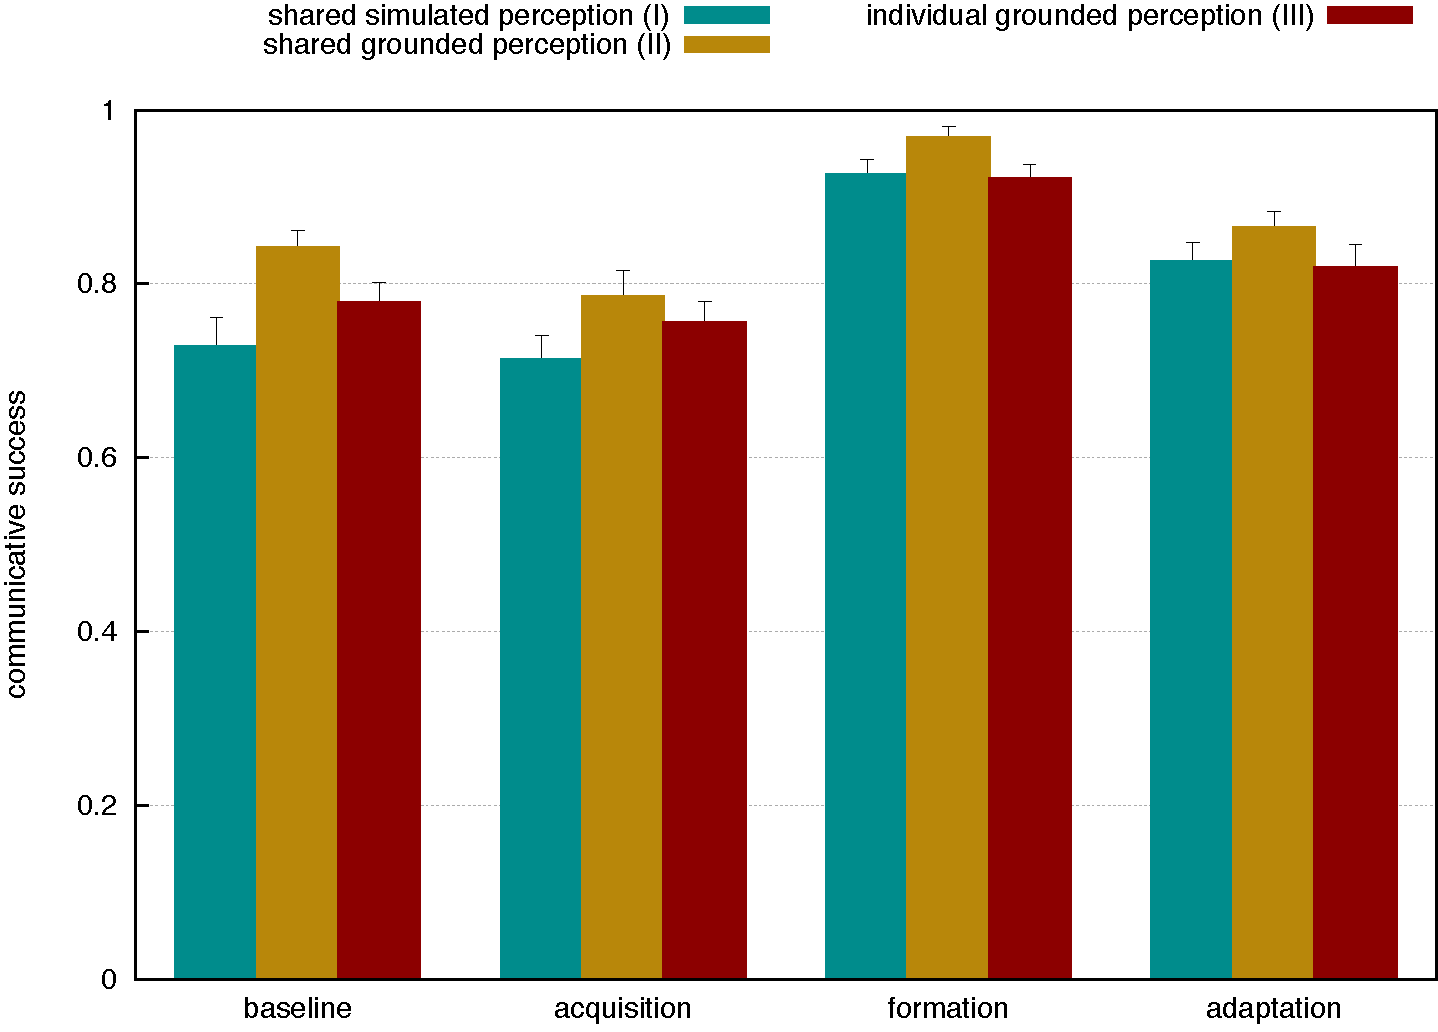
\includegraphics[width=.9\textwidth]{chap11/figs/grounding-comparison.pdf}}
\caption{Comparison of three different environmental set-ups (left, right, and middle columns)
and four different learning conditions. Communicative success is shown on the y-axis.}
\label{fig:grounding-comparison} 
\end{figure}

Interestingly, the best results in terms of communicative success
are obtained when the agents are allowed to evolve their own colour language, 
partly because there was no limit on the number of prototypes they could introduce. This was better 
than using the set of basic colour prototypes for English, simply because English would turn to more complex expressions
(such as \textit{bluish green}) when the basic colour categories are not effective. Moreover, 
agents still achieve better results compared to the English colour system when they do not need to stick 
dogmatically to it. Indeed this shows why alignment, which is widely observed
in human dialogues,\footnote{See: \cite{Garrod:1987} and \cite{Galantucci:2005}.}
is a good strategy for achieving more successful communication.

\section{Conclusion}

This chapter has introduced two major advances with respect to the original Talking Heads experiment: 
the use of semiotic networks to build a more sophisticated mapping between sensory experiences and words, and the 
introduction of language strategies. Each language strategy pairs a particular way of conceptualising reality 
with a particular method to express it using lexicon or grammar. 
These developments were illustrated through several experiments with humanoid robots. Each of these experiments 
was a major step forward in terms of the use of 
highly sophisticated humanoid robots with many degrees of freedom and sophisticated visual processing, grounded compositional 
semantics for the meaning of utterances, and a full-fledged formalism for grammar. 


